\documentclass{article}
\usepackage{amsmath, amssymb}
\usepackage{pgfplots}
\usepackage{mathrsfs}
\usepackage{enumitem}
\usepackage{graphicx} % For \scalebox
\usepackage{hyperref}



\title{MATH 476 Portfolio}
\author{Andres Rocha}
\date{\today}
\usepackage{amsmath, amssymb} % For mathematical symbols and environments
\usepackage{siunitx}
\usepackage{amsmath}
\newcommand{\decrease}{\ensuremath{\text -}}

\begin{document}

\maketitle

\section{Problem Set 1}


\subsection{Notation}

\subsubsection{Definition 1: Delivery Price or Strike Price}
\begin{description}
    \item[\textit{Description of the term:}] Purchase price agreed by long position.
    \item[\textit{Symbol(s):}] $K$
    \item[\textit{Formal Definition:}] The delivery price of the forward contract.
\end{description}


\subsubsection{Definition 2: Spot Price}

\begin{description}
    \item[\textit{Description of the term:}] Purchase price agreed by long position at time T.
    \item[\textit{Symbol(s):}] $S_T$
    \item[\textit{Formal Definition:}] Spot price of the asset at maturity of the contract.
\end{description}

% Add more definitions as needed

\subsection*{Exercise 1}

\textbf{Question:} Find the payoff from a long position in a forward contract and the payoff from a short position in a forward contract on one unit of an asset.

\textbf{Solution:} 
\begin{itemize}
    \item The payoff from a long position in a forward contract on one unit of an asset is $S_T - K$.
    \item The payoff from a short position in a forward contract on one unit of an asset is $K - S_T$.
\end{itemize}


\subsection*{Exercise 2}

\textbf{Question:} Suppose that the S\&R 500 index has a current price of \$1000, and the 6-month forward price is \$1020. What happens if the index price is \$950 in 6 months? \$1200 in 6 months? Construct payoff diagrams for the long and short position on this contract. What would be an advantage of using the forward contract to buy the index in 6 months, as opposed to buying it outright at time t = 0?

\textbf{Solution:}

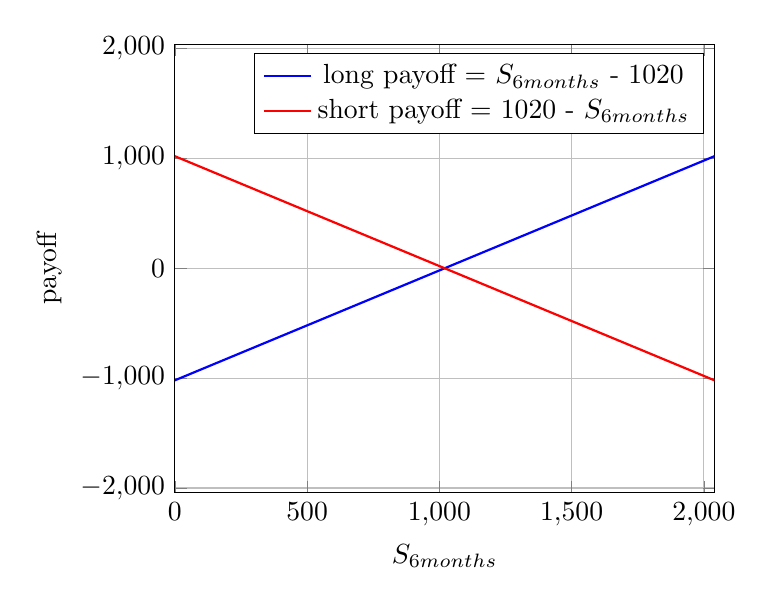
\begin{tikzpicture}
\begin{axis}[
    xlabel=$S_{6 months}$,
    ylabel=payoff,
    xmin=0, xmax=2040,
    ymin=-2040, ymax=2040,
    grid=both,
    ]
    \addplot[domain=0:2040, samples=100, thick, blue]{x - 1020};
    \addplot[domain=0:2040, samples=100, thick, red]{1020 - x};
    \addlegendentry{long payoff = $S_{6 months}$ - 1020}
    \addlegendentry{short payoff = 1020 - $S_{6 months}$}
\end{axis}
\end{tikzpicture}

 \begin{itemize}
     \item If $S_t = \$950$, the payoff for the long position is \$950 - \$1020 = -\$70
 \end{itemize}

  \begin{itemize}
     \item If $S_t = \$950$, the payoff for the short position is \$1020 - \$950 = \$70
 \end{itemize}

 \begin{itemize}
     \item If $S_t = \$1200$, the payoff for the long position is \$1200 - \$1020 = \$180
 \end{itemize}

  \begin{itemize}
     \item If $S_t = \$1200$, the payoff for the short position is \$1020 - \$1200 = -\$180
 \end{itemize}

\noindent \textbf{\textit{The advantage of the forward contract is that you are guaranteed a future price to buy the asset at}}.


\subsection*{Exercise 3}

\textbf{Question:} Construct payoff diagrams for the long and short positions in a forward contract with delivery price K and spot price $S_T$

\textbf{Solution:}

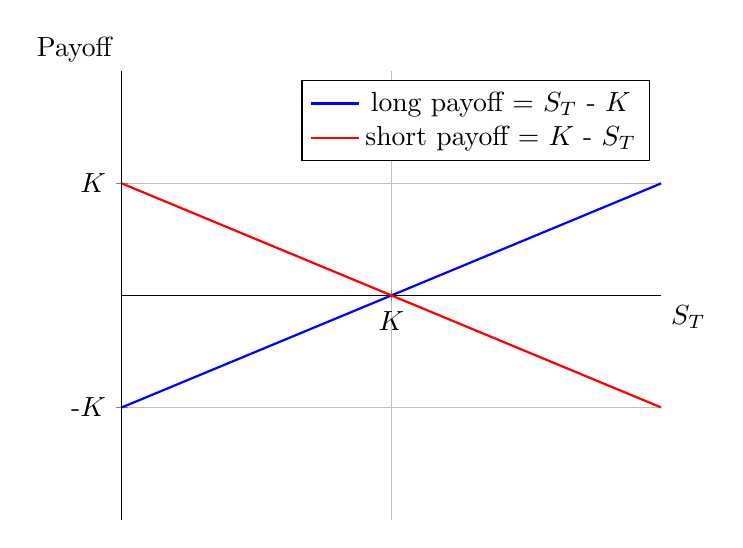
\begin{tikzpicture}
\begin{axis}[
    xlabel=$S_T$,
    ylabel= Payoff,
    axis lines=middle,
    axis line style={-},
    xlabel style={below right},
    ylabel style={above left},
    xmin=0, xmax=2040,
    ymin=-2040, ymax=2040,
    xtick={1020},
    ytick={-1020, 1020},
    xticklabels={$K$},
    yticklabels={-$K$, $K$},
    grid=both,
    ]
    \addplot[domain=0:2040, samples=100, thick, blue]{x - 1020};
    \addplot[domain=0:2040, samples=100, thick, red]{1020 - x};
    \addlegendentry{long payoff = $S_T$ - $K$}
    \addlegendentry{short payoff = $K$ - $S_T$}

\end{axis}
\end{tikzpicture}

\subsection*{Exercise 4}

\textbf{Question:}  Forward contracts on foreign exchange are very popular. Most large banks employ both spot and forward foreign-exchange traders. The table below shows quotes for the exchange rate between the British pound (GBP) and the U.S. dollar (USD) in May 2020. The quote is for the number of USD per GBP.

\begin{table}[htbp]
  \centering
  \label{tab:example}
  \begin{tabular}{|c|c|c|}
    \hline
     & Bid & Ask \\
    \hline
    Spot & 1.2217 & 1.2220  \\
    \hline
    1-month forward & 1.2218 & 1.2222 \\
    \hline
    3-month forward & 1.2220 & 1.2225 \\
    \hline
    6-month forward & 1.2224 & 1.2230 \\
    \hline
  \end{tabular}
\end{table}

\noindent Suppose that the treasurer of a US corporation knows it will pay 1 million in GBP in 6 months and wants to hedge against exchange rate changes. Suppose that the bank agrees to a 6-month forward contract to purchase 1 million GBP in 6 months. (i) What happens if the spot exchange rate is 1.3000 in 6 months? (ii) What is the sport exchange rate is 1.2000 in 6 months?

\textbf{Solution:}

(i) If the spot exchange rate is 1.3000 in 6 months, given the asking price of 

1.2230, the Treasurer's payoff is:

\vspace{\baselineskip}

\indent (Spot Price) - (Delivery Price), the long position

\vspace{\baselineskip}

\indent = (1000000 GBP × 1.30 USD/GBP) - (1000000 GBP × 1.2230 USD/GBP) 

\vspace{\baselineskip}

= 77000 USD 

\vspace{\baselineskip}

(ii) If the spot exchange rate is 1.2000 in 6 months, given the asking price of

1.2230, the Treasurer's payoff is:

\vspace{\baselineskip}

\indent (Spot Price) - (Delivery Price), the long position

\vspace{\baselineskip}

\indent = (1000000 GBP × 1.20 USD/GBP) - (1000000 GBP - 1.2230 USD/GBP) 

\vspace{\baselineskip}

= -23000 USD



\subsection*{Exercise 5}

\textbf{Question:} An investor enters into a short forward contract to sell 100,000 British Pounds for U.S dollars at an exchange rate of 1.3000 USD per pound. How much does the investor gain or lose if the exchange rate at the end of the contract is (i) 1.2900 and (ii) 1.3200?

\textbf{Solution:}

(i) If the exchange rate at the end of the contract is 1.2900 then the investor's 

payoff would be:

\vspace{\baselineskip}

(Delivery Price) - (Spot Price), the short position

\vspace{\baselineskip}

= (100,000 GBP x 1.3 USD/GBP) - (100,000 GBP x 1.29 USD/GBP)

\vspace{\baselineskip}

= 1000 USD

\vspace{\baselineskip}

(ii) If the exchange rate at the end of the contract is 1.2900 then the investor's 

payoff would be:

\vspace{\baselineskip}

(Delivery Price) - (Spot Price), the short position

\vspace{\baselineskip}

= (100,000 GBP x 1.3 USD/GBP) - (100,000 GBP x 1.32 USD/GBP)

\vspace{\baselineskip}

= -2000 USD


\subsection*{Exercise 6}

\textbf{Question:} A trader enters into a short forward contract on 100 million yen. The forward exchange rate is \$0.0090 per yen. How much does the trader gain or lose if the exchange rate at then end of the contract is (i) \$0.0084 per yen and (ii) \$0.0101.

\textbf{Solution:}

(i) If the exchange rate at the end of the contract is \$0.0084 per yen

the investors payoff is:

\vspace{\baselineskip}

(Delivery Price) - (Spot Price), the short position

\vspace{\baselineskip}

= (100 Million Yen x 0.0090 USD/YEN) - (100 Million Yen x 0.0089 USD/YEN)

\vspace{\baselineskip}

= 60,000 USD

(ii) If the exchange rate at the end of the contract is \$0.0101 per yen

the investors payoff is:

\vspace{\baselineskip}

(Delivery Price) - (Spot Price), the short position

\vspace{\baselineskip}

= (100 Million Yen x 0.0090 USD/YEN) - (100 Million Yen x 0.0101 USD/YEN)

\vspace{\baselineskip}

= -110,000 USD

\subsection*{Exercise 7}

\textbf{Question:} Consider the following European call option. Let T denote the date exctly 10
days from now. At time T, the holder of the option may purchase one share of XYZ stock for \$250. To gain an understanding of how call options work and what might be reasonable for the price of this option, we will consider two possible situations that might occur on the expiry time T. Let $S_T$ denote the price of one share of XYZ stock at time T. (i) What happens if $S_{10days}$ = \$270 ? (ii) What happens if $S_{10days}$ = \$230 ?

\textbf{Solution:}

(i)
If $S_{10 days}$ $=$ $\$270$ then the payoff is,
\vspace{\baselineskip}

max[\$0, $S_{10 days}$ - $K$] ; the holder is in the long position
\vspace{\baselineskip}

= max[\$0, \$270 - \$250]
\vspace{\baselineskip}

= max[\$0, \$20]
\vspace{\baselineskip}

= \$20

$\therefore$ the holder uses his right to buy the stock 

\vspace{\baselineskip}

(ii)
If $S_{10 days}$ $=$ $\$230$ then the payoff is,
\vspace{\baselineskip}

max[0, $S_{10 days}$ - $K$] ; the holder is in the long position
\vspace{\baselineskip}

= max[0, \$230 - \$250]
\vspace{\baselineskip}

= max[0, -\$20]
\vspace{\baselineskip}

= \$0

$\therefore$ the holder does not use his right to buy the stock 

\subsection*{Exercise 8}

\textbf{Question:} Suppose that the XYZ share in example 7 only takes the values \$230 or \$270 with equal probability. Find the expected payoff at time T on the call option. This expected value is a useful approximation for what a reasonable amount to pay for the call option would be.

\textbf{Solution:}

$\mathscr{E} = \frac{1}{2} \cdot \$20 + \frac{1}{2} \cdot \$0 = \$10$

\subsection*{Exercise 9}

\textbf{Question:} Let c denote the expected payoff that you obtained in Exercise 8. Although option pricing is, in general, more complicated, suppose that the holder of the option did pay c for this option:

(i) What is his net profit or loss if $S_{10 days}$ = \$270? Express the net profit 

or loss in this case as a percentage of the initial cost of the option.

(ii) What is his net profit or loss if $S_{10 days}$ = \$230? Express the net profit 

or loss in this case as a percentage of the initial cost of the option.

\textbf{Solution:}

(i)
If $S_{10 days}$ = \$270 then the profit is,

\vspace{\baselineskip}

max[\$0, $S_{10 days}$ - $K$] - c

\vspace{\baselineskip}

= max[\$0, \$270 - \$250] - \$10 ; holder is in the long position 

\vspace{\baselineskip}

= max[\$0, \$20] - \$10

\vspace{\baselineskip}

= \$20 - \$10

\vspace{\baselineskip}

= \$10

$\therefore$ since $\$10 / \$10$ = 100\%, the gain is 100\% of the initial cost 
\vspace{\baselineskip}

(ii)
If $S_{10 days}$ = \$230 then the profit is,

\vspace{\baselineskip}

max[\$0, $S_{10 days}$ - $K$] - c ; holder is in the long position 

\vspace{\baselineskip}

= max[\$0, \$230 - \$250] - \$10

\vspace{\baselineskip}

= max[\$0, -\$20] - \$10

\vspace{\baselineskip}

= \$0 - \$10

\vspace{\baselineskip}

= -\$10

$\therefore$ since $-\$10 / \$10$ = -100\%, the loss is 100\% of the initial cost 

\subsection*{Exercise 10}

\textbf{Question:} Suppose that, instead, the investor purchased the share for \$250 instead of purchasing the option.Express his net profit or loss in each case (i.e. (i) $S_{10 days}$ = \$230 or (ii) $S_{10 days}$ = \$270) as a percentage of the initial cost of purchasing the share. Compare with the results of the previous exercise:

\vspace{\baselineskip}

\textbf{Solution:}

(i)
If $S_{10 days}$ = \$230 the profit is,

\vspace{\baselineskip}

$S_{10days}$ - $K$ ; the investor is taking the long position

\vspace{\baselineskip}

= \$230 - \$250 

\vspace{\baselineskip}

= -\$20

$\therefore$ since -\$20/\$250 = -8\% the investor loses 8\% of the initial cost

\vspace{\baselineskip}

(ii)
If $S_{10 days}$ = \$270 the profit is,

\vspace{\baselineskip}

$S_{10days}$ - $K$ ; the investor is taking the long position

\vspace{\baselineskip}

= \$270 - \$250 

\vspace{\baselineskip}

= \$20

$\therefore$ since \$20/\$250 = 8\% the investor gains 8\% of the initial cost

\subsection*{Exercise 11}

\textbf{Question:} Consider an investor who but a European put option to sell 100 shares of stock XYZ with a strike price of \$70. Suppose that the current stock price is (i)\$65. (ii) What happens if $S_T$ = \$55?

\textbf{Solution:}

The holder of the EPO has the right to sell the asset at the strike price.

\vspace{\baselineskip}

(i) If $S_T$ = \$65 the holder of the EPO will use his right to sell the option 

for \$70 per share. The payoff is,

\vspace{\baselineskip}

($K$ - $S_T$) $\cdot$ 100 ; the holder has the long position

\vspace{\baselineskip}

= (\$70 - \$65) $\cdot$ 100

\vspace{\baselineskip}

= \$500

\vspace{\baselineskip}

(ii) If $S_T$ = \$55 the holder of the EPO will use his right to sell the option 

for \$70 per share. The payoff is,

\vspace{\baselineskip}

($K$ - $S_T$) $\cdot$ 100 ; the holder has the long position 

\vspace{\baselineskip}

= (\$70 - \$55) $\cdot$ 100

\vspace{\baselineskip}

= \$1500

\subsection*{Exercise 12}

\textbf{Question:} It is important to observe that sometimes an investor chooses to exercise an option even though
he may make a loss overall. For example, suppose that an investor buys a European call option with a strike
price of \$100 per share to buy 100 shares of XYS stock, and that the current stock price is \$98 per share. The price of the option to purchase these 100 shares is \$500. Suppose that the price of the stock is \$102 per share at expiry. Explain why it is preferable for the investor to exercise the option in this case, even though he makes a loss overall.

\textbf{Solution:}

There are two cases:


(i) The investor buys XYS stock at expiry 

(ii) The investor does not buy XYS stock at expiry

\vspace{\baselineskip}

(i)

$Profit_1$ = $S_{expiry}$ - $K$ - (initial cost); investor has the long position

\hspace{1.1cm}= 100 $\cdot$ (\$102 - \$100) - \$500

\hspace{1.1cm}= -\$300


(ii)

$Profit_2$  = $S_{expiry}$ - $K$ - (initial cost); investor has the long position

\hspace{1.1cm}= 100 $\cdot$ (0 - \$100)

\hspace{1.1cm}= -\$10000

$\therefore$ It is preferable to exercise the option to minimize the loss.

\subsection*{Exercise 13}

\textbf{Question:} Find each of the following:

\vspace{\baselineskip}

(i) The payoff to the holder of a long position in a European call option.

\vspace{\baselineskip}

(ii) The payoff to the holder of a short position in a European call option.

\vspace{\baselineskip}

(iii) The payoff to the holder of a long position in a European put option.

\vspace{\baselineskip}

(iv) The payoff to the holder of a short position in a European put option

\textbf{Solution:}

(i) Payoff = max[\$0, $S_T$ - $K$]

(ii) Payoff = -max[\$0, $S_T$ - $K$] 

(iii) Payoff = max[\$0, $K$ - $S_T$]

(iv) Payoff = -max[\$0, $K$ - $S_T$]

\subsection*{Exercise 14}

\textbf{Question:} Construct payoff diagrams for each of the four positions above (long call, short call, long pout, short put).

\textbf{Solution:} 

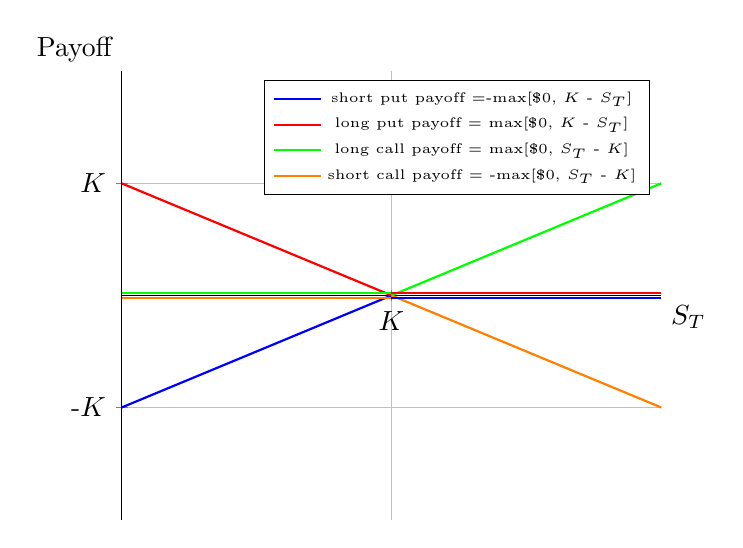
\begin{tikzpicture}
\begin{axis}[
    xlabel=$S_T$,
    ylabel= Payoff,
    axis lines=middle,
    axis line style={-},
    xlabel style={below right},
    ylabel style={above left},
    xmin=0, xmax=2040,
    ymin=-2040, ymax=2040,
    xtick={1020},
    ytick={-1020, 1020},
    xticklabels={$K$},
    yticklabels={-$K$, $K$},
    grid=both,
    legend style={font=\tiny},
    ]
    \addplot[domain=0:1020, samples=100, thick, blue]{x - 1020};
    \addplot[domain=0:1020, samples=100, thick, red]{1020 - x};=

    \addplot[domain=1020:2040, samples=100, thick, green]{x - 1020};
    \addplot[domain=1020:2040, samples=100, thick, orange]{1020 - x};
    \addplot[domain=0:1020, samples=100, thick, green]{20};
    \addplot[domain=0:1020, samples=100, thick, orange]{-20};

    \addplot[domain=1020:2040, samples=100, thick, red]{20};
    \addplot[domain=1020:2040, samples=100, thick, blue]{-20};
    
    \addlegendentry[draw=none]{short put payoff =-max[\$0, $K$ - $S_T$]}
    \addlegendentry[draw=none]{long put payoff = max[\$0, $K$ - $S_T$]}
    \addlegendentry[draw=none]{long call payoff = max[\$0, $S_T$ - $K$]}
    \addlegendentry[draw=none]{short call payoff = -max[\$0, $S_T$ - $K$]}

\end{axis}
\end{tikzpicture}

\subsection*{Exercise 15}

\textbf{Question:} An investor buys a European put on a share for \$3. The stock price is \$42, and the strike price is \$40. Under what circumstances does the investor make a profit? Under what circumstances will the option be exercised? Draw a profit diagram illustrating the variation of the investor’s profit (not the payoff) with the stock price at the maturity of the option.

\textbf{Solution:} 

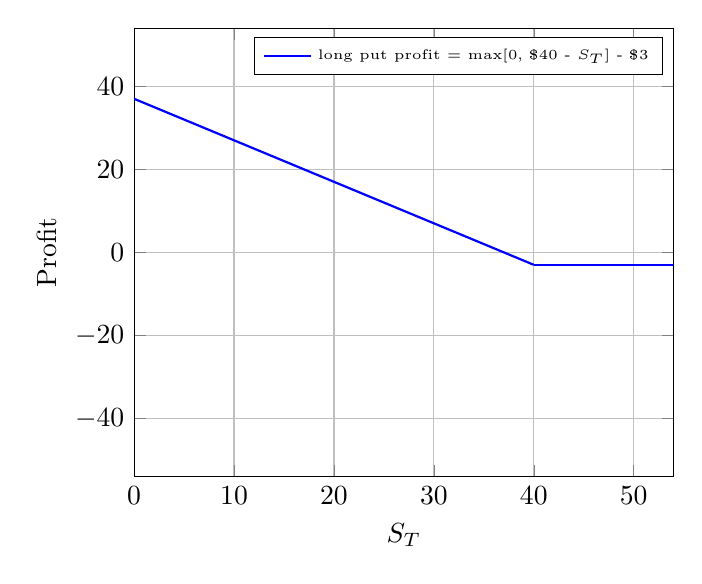
\begin{tikzpicture}
\begin{axis}[
    xlabel=$S_T$,
    ylabel=Profit,
    xmin=0, xmax=54,
    ymin=-54, ymax=54,
    grid=both,
    legend style={font=\tiny},
    ]
    \addplot[domain = 0:40, samples=100, thick, blue]{37 - x};
    \addplot[domain = 40:54, samples=100, thick, blue]{-3};
    \addlegendentry{long put profit = max[0, \$40 - $S_T$] - \$3}
\end{axis}
\end{tikzpicture}

The investor will exercise the option if $S_T$ $<$ 37 (x intercept), else the investor will choose 

not to exercise the option.

\subsection*{Exercise 16}

\textbf{Question:} An investor sells a European call on a share for \$4. The stock price is \$47, and the strike price is
\$50. Under what circumstances does the investor make a profit? Under what circumstances will the option be
exercised? Draw a diagram showing the variation of the investor’s profit with the stock price at the maturity of
the option.

\textbf{Solution:} 

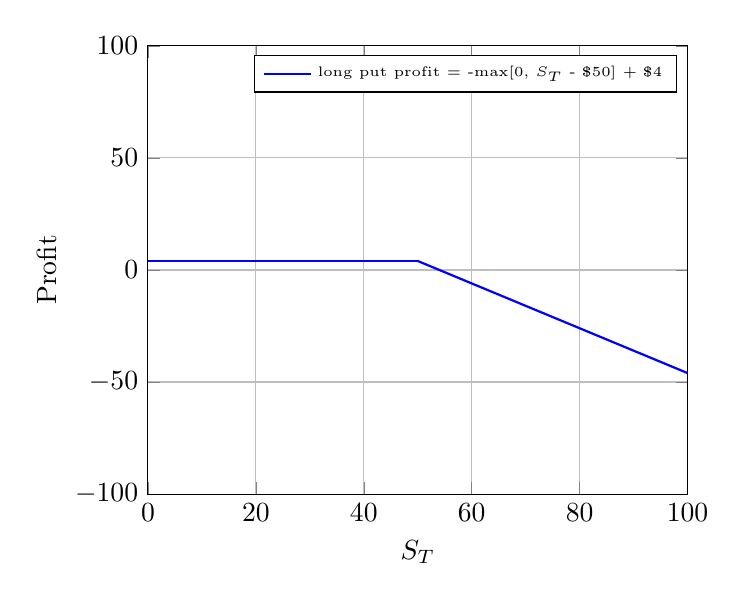
\begin{tikzpicture}
\begin{axis}[
    xlabel=$S_T$,
    ylabel=Profit,
    xmin=0, xmax=100,
    ymin=-100, ymax=100,
    grid=both,
    legend style={font=\tiny}
    ]
    \addplot[domain = 50:100, samples=100, thick, blue]{54 - x};
    \addplot[domain = 0:50, samples=100, thick, blue]{4};
    \addlegendentry{long put profit = -max[0,  $S_T$ - \$50] + \$4}
\end{axis}
\end{tikzpicture}

The investor will profit if the $S_T$ $<$ \$54. (x-intercept)

\subsection*{Exercise 17}

\textbf{Question:} An investor sells a European call option with strike price K and maturity T , and buys a put with
the same strike price and maturity. Describe the investor’s position–describe all of the possible situations at
maturity, explain which (if any) of the options the investor should exercise at maturity, and find the investor’s
payoff in each case.


\textbf{Solution:} 


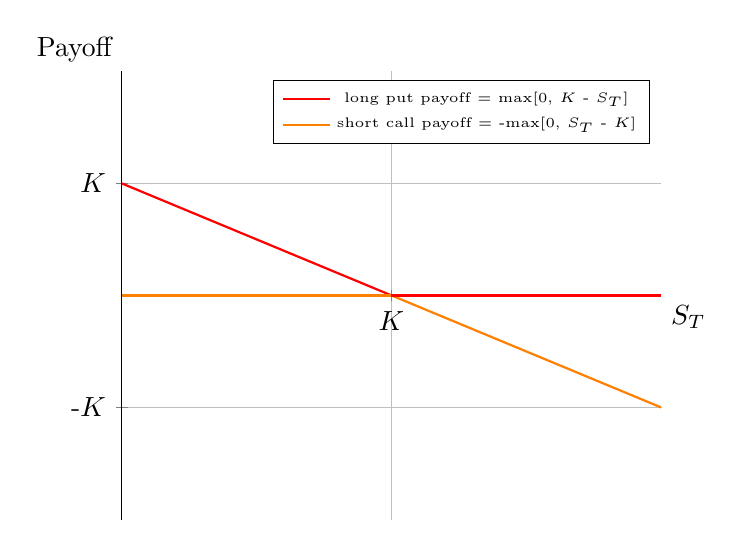
\begin{tikzpicture}
\begin{axis}[
    xlabel=$S_T$,
    ylabel= Payoff,
    axis lines=middle,
    axis line style={-},
    xlabel style={below right},
    ylabel style={above left},
    xmin=0, xmax=2040,
    ymin=-2040, ymax=2040,
    xtick={1020},
    ytick={-1020, 1020},
    xticklabels={$K$},
    yticklabels={-$K$, $K$},
    grid=both,
    legend style={font=\tiny},
    ]

    \addplot[domain=0:1020, samples=100, thick, red]{1020 - x};=

    \addplot[domain=1020:2040, samples=100, thick, orange]{1020 - x};
    \addplot[domain=0:1020, samples=100, thick, orange]{0};

    \addplot[domain=1020:2040, samples=100, thick, red]{0};
    
    \addlegendentry[draw=none]{long put payoff = max[0, $K$ - $S_T$]}
    \addlegendentry[draw=none]{short call payoff = -max[0, $S_T$ - $K$]}

\end{axis}
\end{tikzpicture}

This is the same as if the investor took the short position in a forward 

contract. In other words $K$ - $S_T$, the short position in a forward contract.


\subsection*{Exercise 18}

\textbf{Question:} A trader buys a call option with a strike price of \$45 and a put option with a strike price of \$40.
Both options have the same maturity. The call costs \$3 and the put costs \$4. Draw a diagram showing the
variation of the trader’s profit with the asset price. Note: this type of trading strategy is known as a strangle.

\textbf{Solution:} 

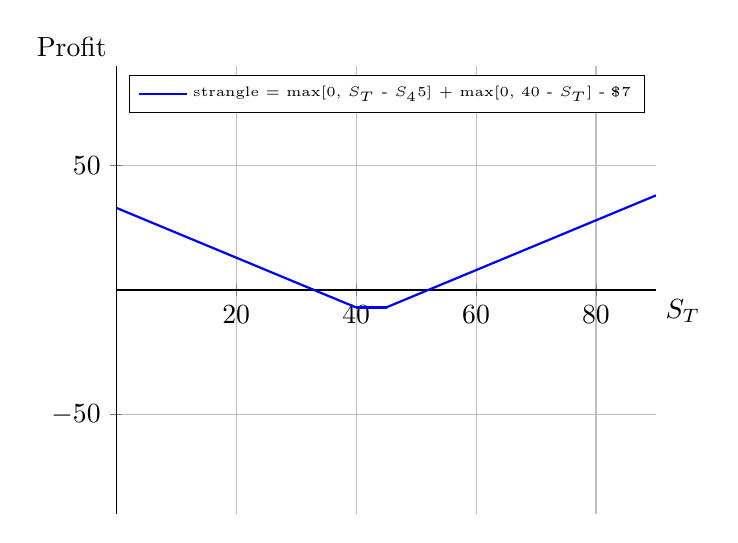
\begin{tikzpicture}
\begin{axis}[
    xlabel=$S_T$,
    ylabel= Profit,
    axis lines=middle,
    axis line style={-},
    xlabel style={below right},
    ylabel style={above left},
    xmin=0, xmax=90,
    ymin=-90, ymax=90,
    grid=both,
    legend style={font=\tiny},
    ]

    \addplot[domain=0:40, samples=100, thick, blue]{33 - x};
    \addplot[domain=40:45, samples=100, thick, blue]{-7};
    \addplot[domain=45:90, samples=100, thick, blue]{x - 52};
    
    \addlegendentry[draw=none]{strangle = max[0, $S_T$ - $S_45$] +  max[0, $40$ - $S_T$] - \$7}

\end{axis}
\end{tikzpicture}

\, A strangle is a good strategy for volatile assets 

\subsection*{Exercise 19}

\textbf{Question:} Explain why an American option is always worth at least as much as a European option on the
same asset with the same strike price and exercise date.

\textbf{Solution:} 
Let's suppose that the American option was worth less then the 

European option in some instance where the strike price and expiry date 

were the same. If we can show that this makes no sense then it will explain 

why the American option is always worth at least as much a European 

option.

\vspace{\baselineskip}

- The American option gives the holder the right to buy or sell an asset 

before and including at the expiry date

- The European option gives the holder the right to buy or sell an asset at 

the expiry date. 

\vspace{\baselineskip}

If the American option was worth less then the European option this would 

not make sense, since your are paying less for more rights on when to buy 

or sell the asset on top of already being able to buy or sell at the expiry 

date. 

\subsection*{Exercise 20}

\textbf{Question:} Complete the following table to summarize the effect on the price of a stock option of increasing
one variable while keeping all others fixed. Write a "+" to indicate that an increase in the variable causes the option
price to increase, and write a "-" to indicate that an increase in the variable causes the option price to decrease.
Write a ? if the relationship is uncertain.

\newpage

\begin{table}
    \centering
    \begin{tabular}{|c|c|c|c|c|} \hline 
         Variable&  European Call&  European Put&  American Call& American Put\\ \hline 
         Current Price&  +&  -&  +& -\\ \hline 
         Stock Price&  -&  +&  -& +\\ \hline 
         Time to expiration&  +&  +&  +& +\\ \hline 
         Volatility&  +&  +&  +& +\\ \hline 
         Risk-free interest rate&  +&  ?&  +& ?\\ \hline
    \end{tabular}
 
\end{table}

\subsection*{Exercise 21}

\textbf{Question:} A trader writes a December put option with a strike price of \$30. The price of the option is \$4.
Under what circumstances does the trader make a profit?

\textbf{Solution:} 

The profit is,

\vspace{\baselineskip}

max[\$0, $K$ - $S_T$] - \$4 ; the writer has the short position

\vspace{\baselineskip}

= -max[0, \$30 - $S_T$] + \$4

\vspace{\baselineskip}

$\therefore$ the trader makes profit if $S_T$ $>$ \$26 

\subsection*{Exercise 22}

\textbf{Question:} Suppose that a March call option to buy a share for \$50 costs \$2.50 and is held until March. Under
what circumstances will the holder of the option make a profit? Under what circumstances will the option be
exercised? Draw a diagram illustrating how the profit from a long position in the option depends on the stock
price at maturity of the option.

\textbf{Solution:} 

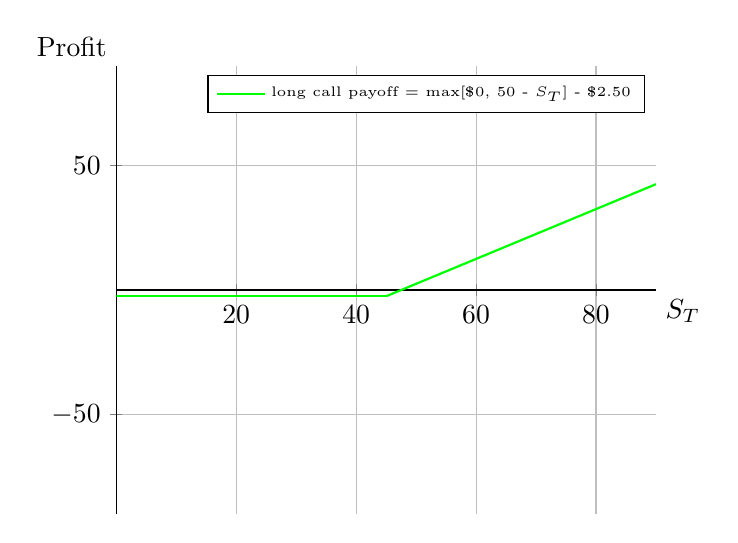
\begin{tikzpicture}
\begin{axis}[
    xlabel=$S_T$,
    ylabel= Profit,
    axis lines=middle,
    axis line style={-},
    xlabel style={below right},
    ylabel style={above left},
    xmin=0, xmax=90,
    ymin=-90, ymax=90,
    grid=both,
    legend style={font=\tiny},
    ]

    \addplot[domain=45:90, samples=100, thick, green]{x - 47.50};
    \addplot[domain=0:45, samples=100, thick, green]{-2.50};

    
    \addlegendentry[draw=none]{long call payoff = max[\$0, $50$ - $S_T$] - \$2.50}

\end{axis}
\end{tikzpicture}

The option will not be exercised if $S_T$ $<$ \$47.50. If $S_T$ $>$ \$47.50 the option 

will be exercised. Note that \$47.50 is the x-intercept.

\subsection*{Exercise 23}

\textbf{Question:} It is May and a trader writes a September call option with a strike price of \$20. The stock price is \$18 and the option price is \$2. Describe the trader’s cash flows if the option is held until September and the
stock price is \$25 at that time.

\textbf{Solution:} 

If $S_{September}$ = \$25,

\vspace{\baselineskip}

The profit is,

\vspace{\baselineskip}

-max[\$0, $S_T$ - $K$] - (initial cost) ; the writer has the short position 

\vspace{\baselineskip}

= -max[\$0, \$25 - \$20] + \$2

\vspace{\baselineskip}

= -\$3

\vspace{\baselineskip}

and the payoff is \$5.

\subsection*{Exercise 24}

\textbf{Question:} Trader A enters into a forward contract to buy an asset for \$1,000 in one year. Trader B buys a
call option to buy the asset for \$1,000 in one year. The cost of the option is \$100. What is the difference between the positions of the traders? Show the profit as a function of the price of the asset in one year for the two traders.

\textbf{Solution:} 

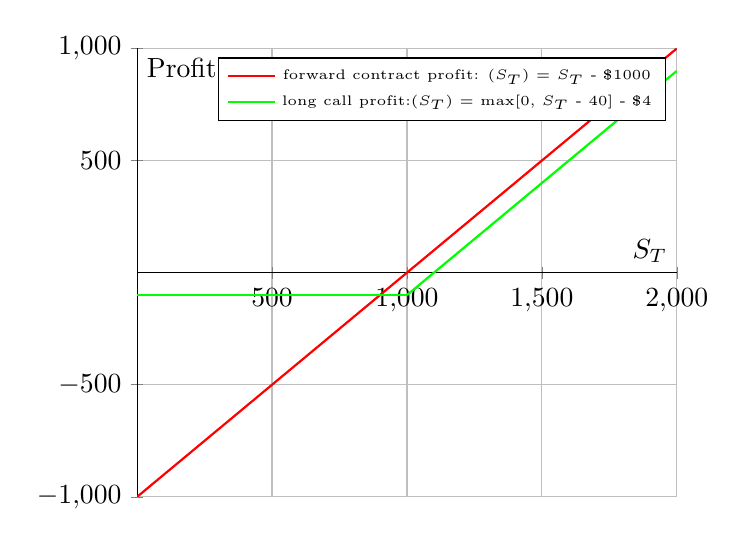
\begin{tikzpicture}
\begin{axis}[
    xlabel=$S_T$,
    ylabel= Profit,
    axis lines=middle,
    axis line style={-},
    xmin=0, xmax=2000,
    ymin=-1000, ymax=1000,
    grid=both,
    legend style={font=\tiny},
    ]

    \addplot[domain=0:2000, samples=100, thick, red]{x - 1000};

    \addplot[domain=1000:2000, samples=100, thick, green]{x - 1100};
    \addplot[domain=0:1000, samples=100, thick, green]{-100};

    
    \addlegendentry[draw=none]{forward contract profit: ($S_T$) = $S_T$ - \$1000}
    \addlegendentry[draw=none]{long call profit:($S_T$) = max[0, $S_T$ - $40$] - \$4}

\end{axis}
\end{tikzpicture}

The main difference between the positions is that Trader A is taking on 

more risk to losses compared to Trader B in exchange for the possibility of 

higher profits.

\subsection*{Exercise 25}

\textbf{Question:} A trader is considering two alternatives: buy 100 shares of
the stock and buy 100 September call options with a strike price of \$320. For each alternative, find each of the
following (i) the upfront cost, (ii) the total profit if the stock price in September is \$400, and (iii) the total loss if the stock price in September is \$300. With the cost of a single option being \$21.70.

\textbf{Solution:} 

(i) 

- If the trader buys 100 shares of stock the upfront cost is;  

\vspace{\baselineskip}

\, (100 Share) $\cdot$ 316.50 (USD/Share) = \$31,650

\vspace{\baselineskip}

- If the trader buys 100 call options the upfront cost is;  

\vspace{\baselineskip}

\, (100 Option) $\cdot$ 21.70 (USD/Option) = \$2,170

\vspace{\baselineskip}

(ii)

- If the trader buys 100 shares and $S_T$ = \$400 the profit is;

\vspace{\baselineskip}

\, 100 $\cdot$ ($S_{September}$ - $K$) 

\vspace{\baselineskip}

\, = 100 $\cdot$ (\$400 - \$320)

\vspace{\baselineskip}

\, = \$8000

\vspace{\baselineskip}

- If the trader buys 100 options and $S_T$ = \$400 the profit is;

\vspace{\baselineskip}

\, 100 $\cdot$ (max[\$0, $S_{September}$ - $K$]  - (initial cost))

\vspace{\baselineskip}

\, = 100  $\cdot$ (max[\$0, \$400 - \$320]  - \$21.70)

\vspace{\baselineskip}

\, = \$5830

\vspace{\baselineskip}

(iii)

- If the trader buys 100 shares and $S_T$ = \$400 the profit is;

\vspace{\baselineskip}

\, 100 $\cdot$ ($S_{September}$ - $K$) 

\vspace{\baselineskip}

\, = 100 $\cdot$ (\$300 - \$320)

\vspace{\baselineskip}

\, = -\$2000

\vspace{\baselineskip}

- If the trader buys 100 options and $S_T$ = \$300 the profit is;

\vspace{\baselineskip}

\, 100 $\cdot$ (max[0, $S_{September}$ - $K$]  - (initial cost))

\vspace{\baselineskip}

\, = 100  $\cdot$ (max[0, \$300 - \$320]  - \$21.70)

\vspace{\baselineskip}

\, = -\$2170

\subsection*{Exercise 26}

\textbf{Question:} On May 21, 2020, an investor owns 100 Apple shares. The
investor is comparing two alternatives to limit risk. The first involves buying one December put option contract
 at \$3.30 with a strike price of \$290. The second involves instructing a broker to sell the 100 shares as soon as Apple’s
price reaches \$290. Discuss the advantages and disadvantages of the two strategies.

\textbf{Solution:} 

By choosing the put option contract the most investor can lose is \$3300, 

since that is what is payed 
to be in the long position of the option.

\vspace{\baselineskip}

By choosing the second alternative the investor is making a the 
assumption 

that the asset will reach \$290. This could be more of risk compared to the 

first alternative, depending on what this assumption was based on.

\vspace{\baselineskip}

Therefore, if the goal of the investor is to limit risk then choosing a put 

option contract would be better compared to the other alternative. 

\subsection*{Exercise 27}

\textbf{Question:} Suppose that a deposit of \$150 attracts simple annual interest at a rate of 8\%. Find the value of
the deposit after 20 days. Assume that there are 365 days in one year.

\textbf{Solution:}

The future value of simple annual interest is given by,

\vspace{\baselineskip}

P(1 + tr)

\vspace{\baselineskip}

= \$150 $\cdot$ $(1 + 20/365 * 8/100)$ 

\vspace{\baselineskip}

= \$150.66

\subsection*{Exercise 28}

\textbf{Question:} Find the principal to be deposited initially in an account attracting simple annual interest at a rate
of 8\% if \$1,000 is needed after three months. Assume that there are 12 months in one year.

\textbf{Solution:}

The principal (P) is given by,

\vspace{\baselineskip}

P(1 + tr) = V(t) ; where V(t) is the future value

\vspace{\baselineskip}

= P $\cdot$ $(1 + (31 \cdot 3)/365 \cdot 8/100)$ = \$1000 ; assuming 31 days per month

\vspace{\baselineskip}

$\therefore$ P = \$980.02

\subsection*{Exercise 29}

\textbf{Question:} Find and compare the future value after two years of a deposit of \$100 attracting interest at an
annual interest rate of 10\% is compounded (a) annually and (b) monthly.

\textbf{Solution:}

(a) If the deposit compounds annually, the future value is given by,

\vspace{\baselineskip}

V(t) = P $\cdot$ $(1 + r/m) ^ {tm}$ ; with m = 1

\vspace{\baselineskip}

= \$100 $\cdot$ $(1 + .10/1) ^ {2 \cdot 1}$

\vspace{\baselineskip}

= \$121

\vspace{\baselineskip}

(b) If the deposit compounds monthly, the future value is given by,

\vspace{\baselineskip}

V(t) = P $\cdot$ $(1 + r/m) ^ {tm}$ ; with m = 12

\vspace{\baselineskip}

= \$100 $\cdot$ $(1 + .10/12) ^ {2 \cdot 12}$

\vspace{\baselineskip}

= \$122.03\textbf{}

\subsection*{Exercise 30}

\textbf{Question:} Show that if m $<$ k, then $(1 + r/m) ^ m$ $<$ $(1 + r/k)^k$.
Interpret this in the context of future value (i.e. write a sentence using financial terms that describes what this inequality tells us in terms of future value of money).

\textbf{Solution:}

Define $f$(x) = $(1 + 1/x) ^ x$. If we can show $f^\prime$(x) $>$ 0 then the proof is 

complete, since this would show that f is increasing and therefore by 

definition of an increasing function $f$(m) $<$ $f$(k) since m $<$ k.

\vspace{\baselineskip}

Assuming x is positive since m and k represent the number of interest 

payments,

\vspace{\baselineskip}

$f^\prime$(x) = ln($1 + 1/x$)$($1 + 1/x$) ^ x$  $>$ 0 , since 1 + 1/x $>$  1.

\vspace{\baselineskip}

\textit{The inequality} $(1 + r/m) ^ m$ $<$ $(1 + r/k)^k$ \textit{shows that future values increase }

\textit{along with the number of interest payments. } 

\subsection*{Exercise 31}

\textbf{Question:} In the case of continuously compounded interest, interest is
added continuously to the principal. If V (t) is the amount in the bank at time t and if r is the constant interest
rate, then we obtain the following differential equation for V as a function of t: $dV/dt = r \cdot v$

\vspace{\baselineskip}

\noindent Let P denote the initial principal invested (i.e. P = V (0)), and solve the differential equation above to find a
formula for V as a function of t

\textbf{Solution:}
This is a seperable differential equation. Therefore,

\hspace{0.9cm}$dV/dt$ = rv

$\implies$ $dv/v$ = r dt 

$\implies$ $ln|v(t)|$ = rt + c ; by taking the integral of both sides

$\implies$ $v(t)$ = $e^{rt + c}$ = c$e^{rt}$

\vspace{\baselineskip}

Apply initial condition,

$\implies$ v(0) = c = P

$\therefore$ v(t) = $Pe^{rt}$

\subsection*{Exercise 32}

\textbf{Question:} Continuously compounded interest can also be viewed as period-
ically compounded interest in which we take the limit as m (the number of interest payments made per year)
goes to infinity, i.e.

         \[ V(t) = \lim_{x\to\infty} (1 + r/m) ^ {tm} \cdot  P \]

(a) Show that
         \[ e = \lim_{x\to\infty} (1 + 1/x) ^ x \]

(b) Use the result above and V(t) = $\lim_{x\to\infty} (1 + r/m) ^ {tm} \cdot  P$ to obtain a 

closed form (i.e. without a limit) expression for V (t). You should, of course, 

obtain the same expression that you obtained by solving the differential

equation in Continuous Compounding I.



\textbf{Solution:}

(a)
$\lim_{x\to\infty} (1 + 1/x) ^ x$ , let y = $1/x$

\vspace{\baselineskip}

$\implies$ $\lim_{{y\to 0}} (1 + y) ^ {1/y}$ , rewriting the original limit 

\vspace{\baselineskip}

$\implies$ $\lim_{{y\to 0}} (1 + y) ^ {1/y} = \lim_{{y\to 0}} e^{ln(1+y) ^ {1/y}}$ = $\lim_{{y\to 0}} e^ {1/y \cdot {ln(1+y)}}$

\vspace{\baselineskip}

Now,

\vspace{\baselineskip}

$\lim_{{y\to 0}}  ln(1+y) / y$ $=_{lh} \lim_{{y\to 0}} (1 + y)^ {-1} = 1$

\vspace{\baselineskip}

$\therefore e = \lim_{x\to\infty} (1 + 1/x) ^ x$

(b)

$\lim_{m\to\infty} (1 + r/m) ^ {tm}$ , let y = $1/m$

\vspace{\baselineskip}

$\implies$ $\lim_{{y\to 0}} (1 + ry) ^ {t/y}$ , rewriting the original limit 

\vspace{\baselineskip}

$\implies$ $\lim_{{y\to 0}} (1 + ry) ^ {t/y} = \lim_{{y\to 0}} e^{ln(1+ry) ^ {t/y}}$ = $\lim_{{y\to 0}} e^ {t/y \cdot {ln(1+ry)}}$

\vspace{\baselineskip}

Now taking the limit of the power,

\vspace{\baselineskip}

$\lim_{{y\to 0}}  tln(1+ry) / y$ $=_{lh} \lim_{{y\to 0}} tr (1 + ry)^ {-1} = rt$

\vspace{\baselineskip}

$\therefore Pe^{rt} = \lim_{m\to\infty} P(1 + r/m) ^ {tm}$

\subsection*{Exercise 33}

\textbf{Question:} Show that the stock price is an upper bound on the option price: c $\leq$ $S_0$.
In other words, the option can never be worth more than the stock. 
Hint: Argue that if $S_0$ $<$ c, an arbitrage opportunity exists.
 
\textbf{Solution:}

Assume c $>$ $S_0$ this would imply the option price is worth more than the 

stock price. This leads to a contradiction with the no arbitrage principle 

since the stock could be bought at t=0 and  call option could be sold for a 

guaranteed profit.

\vspace{\baselineskip}

Specifically,

If  $S_T$ $> K$ (the owner of call option exercises the option),

$\implies$ profit = c + K - $S_0$ ; which is clearly positive based on assumption

\vspace{\baselineskip}

If  $S_T$ $\leq$ K (the owner of call option does not exercise the option),

$\implies$ profit = c - $S_0$ ; which is clearly positive based on assumption

$\therefore$  An arbitrage opportunity exists.

\subsection*{Exercise 34}

\textbf{Question:} Show that the put option cannot be worth more than the present value of K today:
$p \leq Ke^{-rT}$.
 
\textbf{Solution:}

Let's suppose for contradiction that $ p > Ke^{-rT} $. This leads to a 

contradiction with the no arbitrage principle, since selling the put option 
is 

a guaranteed profit.

\vspace{\baselineskip}

Specifically,

If  $S_T$ $> K$ (the owner of the put option does not exercises the option),

$\implies$ profit = p - K , which is clearly positive based on assumption

\vspace{\baselineskip}

If  $S_T$ $\leq K$ (the owner of the put option does not exercises the option),

$\implies$ profit = p , which is clearly positive

$\therefore$  An arbitrage opportunity exists.

\subsection*{Exercise 35}

\textbf{Question:} Show that c $\geq$ $S_{0} -Ke^{-rt}$
 
\textbf{Solution:}

Consider two portfolios:

\vspace{\baselineskip}

Portfolio A: One European call option and an amount of cash equal to 

\( Ke^{-rT} \).

Portfolio B: One share of the stock.

\vspace{\baselineskip}

Assume that at time \( T \), the stock price is \( S_T \). The payoff of Portfolio B at 

time \( T \) is simply \( S_T \).

\vspace{\baselineskip}


If \( S_T \geq K \),

- The payoff of portfolio A at time T is, \( S_T - K + K \)

- The payoff of portfolios B is, $S_T$ 

If \( S_T < K \),

- The payoff of portfolio A at time T is, \( K \)

- The payoff of portfolio B is, \( S_T \)



\vspace{\baselineskip}

$\therefore$ Since Portfolio A has a higher or equal to payoff in both scenarios, it must have a 

higher value at time \( T \) than Portfolio B under no-arbitrage conditions, 

directly implying that c $\geq$ $S_{0} -Ke^{-rt}$.

\subsection*{Exercise 36}

\textbf{Question:} Show that p $\geq$ $Ke^{-rt} - S_{0}$
 
\textbf{Solution:}
Consider two portfolios:

\vspace{\baselineskip}

Portfolio A: One European put option and one share of stock.

Portfolio B: K dollars in savings account with a risk free interest rate

\vspace{\baselineskip}

Assume that at time \( T \), the stock price is \( S_T \). The payoff of Portfolio B at 

time \( T \) is simply \( S_T \).

\vspace{\baselineskip}


If \( S_T \geq K \),

- The payoff of portfolio A at time T is, \( Ke^{-rT} - S_T + S_T \)

- The payoff of portfolios B at time T is, $Ke^{-rt}$

If \( S_T < K \),

- The payoff of portfolio A at time T is, \( Ke^{-rT} \)

- The payoff of portfolio B at time T is , \( S_T \)

\vspace{\baselineskip}

$\therefore$ Since Portfolio A has a higher or equal to  payoff in both scenarios, it must 

have a higher value at time \( T \) than Portfolio B under no-arbitrage conditions, 

directly implying that p $\geq$ $Ke^{-rt}$ - $S_{0}$.

\subsection*{Exercise 37}

\textbf{Question:} What is a lower bound for the price of a 2-month European put option on a non- dividend-paying
stock when the stock price is \$58, the strike price is \$65, and the risk- free interest rate is 5\% per annum?
 
\textbf{Solution:}

Using the equation we derived in Exercise 36, p $\geq$ $Ke^{-rt}$ - $S_{0}$.

$\implies p \geq 65 \cdot e^{(-0.05/12) \cdot 2}$ - 58

$\therefore p \geq $ \$6.46

\subsection*{Exercise 38}

\textbf{Question:} Show that c + $Ke^{-rt}$ = p + $S_0$
 
\textbf{Solution:}
Consider two portfolios:

\vspace{\baselineskip}

Portfolio A: One European call option and an amount of cash equal to $Ke^{-rt}$

Portfolio B: One European put option plus one share of the stock 

\vspace{\baselineskip}

If $S_T$ $\geq$ K,

- The payoff of portfolio A at time T is, $S_T$ - $K$ + $K$

- The payoff of portfolio B at time T is, $S_T$

\vspace{\baselineskip}

If $S_T$ $<$ K,

- The payoff of portfolio A at time T is, $K$

- The payoff of portfolio B at time T is, $K$ - $S_T$ + $S_T$

$\therefore$ Since both portfolios are equal are time T,  by the no-arbitrage conditions 

we conclude that c + $Ke^{-rt}$ = p + $S_0$. We call this \textit{put-call parity}.

\subsection*{Exercise 39}

\textbf{Question:} The current price of a stock is $S_0$ = \$19 and the price of a 3-month European call option on the
stock with a strike price of \$20 is \$1. The risk-free annual interest rate is 4\%. What is the price of a 3-month
European put option on the stock with strike price \$20?
 
\textbf{Solution:}
Using the \textit{put-call parity}, c + $Ke^{-rt}$ = p + $S_0$,

$\implies$ p = c + $Ke^{-rt}$ - $S_0$

$\implies$ p = 1 + 20$e^{-(.04/12) \cdot 3}$ - \$19

$\therefore$ p  = \$1.80

\subsection*{Exercise 40}

\textbf{Question:} The prices of European call and put options on a stock with an expiration date in 12 months and
a strike price of \$120 are \$20 and \$5, respectively. The current stock price is \$130. What is the implied risk-free
interest rate?
 
\textbf{Solution:}
Using the \textit{put-call parity}, c + $Ke^{-rt}$ = p + $S_0$,

$\implies$ r = -1/t $\cdot$ ln((p + $S_0$ - c) / k)

$\implies$ r = -ln((5 + 130 - 20)/120)

$\therefore$ p  = 0.0425 

\subsection*{Exercise 41}

\textbf{Question:} Suppose that the price of a stock is \$31, and that the price of a a European call option on the stock
with strike price \$30 is \$3, and that the price of a European put option on the stock with the same strike price
and expiry is \$2.25. The expiry time is 3 months. The risk-free interest rate is 10\% per year. Show that put-call
parity does not hold, and construct an arbitrage opportunity. In particular, show that an arbitrager makes a
risk-free profit by buying the call option and short-selling both the put and the stock.
 
\textbf{Solution:}
Let's substitute the values into the put-call parity equation:

c + $Ke^{-rt}$ = p + $S_0$

$\implies$ $3 + 30 \cdot e^{-(.10/12) \cdot 3)} = 2.25 + 31$

$\implies$ $32.26 \neq 33.25$


$\therefore$ put-call parity does not hold in this case.

\vspace{\baselineskip}
 
An arbitrager can do the following:

\begin{enumerate}
    \item Short sell the put option for \$2.25.
    \item Short sell the stock for \$31.
    \item Buy the call option for \$3.
\end{enumerate}

At the expiration of the options:
\begin{itemize}
    \item If the stock price is above \$30, the call option will be exercised, and the short put will expire worthless. With the stock bought through the call option the arbitrager will close the short sell of the stock.

    profit = [$S_T$ - $S_T$] + [-\$30 - \$3 + \$2.25 + \$31] ; which is positive 
    
    \item If the stock price is below \$30, the put option will be exercised, and the short call will expire worthless. With the stock sold to the arbitrager being in short position of the put option the arbitrager will close the short sell of the stock.

    profit = [$S_T$  - $S_T$] + [-\$30 - \$3 + \$2.25 + \$31] ; which is positive
\end{itemize}

$\therefore$ The arbitrager will profit and therefore makes a risk free profit.

\subsection*{Exercise 42}

\textbf{Question:} A 1-month European put option on a non-dividend-paying stock is currently selling for \$2.50. The stock price is \$47, the strike price is \$50, and the risk-free interest rate is 6\% per annum. What opportunities are there for an arbitrageur?
 
\textbf{Solution:}
Here's how an arbitrageur could exploit this situation:

\begin{enumerate}
    \item \textbf{Borrow \$49.50 at 6\%}: The arbitrageur could borrow the stock at \$49.50 at the risk-free interest rate for one month
    \item \textbf{Buy the Stock}: The arbitrageur could buy the stock at the current market price of \$47
    \item \textbf{Buy the Put Option}: The arbitrageur can buy the put option for \$2.50.
\end{enumerate}

Now, regardless of the value $S_T$ if the arbitrager always exercises their right 

to sell then they always profit since,

\vspace{\baselineskip}

profit = $\$50 - \$49.50e^{.06/12}$ 

$\therefore$ profit = \$0.2525

$\therefore$ The arbitrageur can earn risk-free profit.

\subsection*{Exercise 43}
\textbf{Question:} Explain why the arguments leading to put--call parity for European options cannot be used to give a similar result for American options.

\textbf{Solution.} When early exercise is not possible, we can argue that two portfolios that are worth the same at time $T$ must be worth the same at earlier times. When early exercise is possible, the argument is no longer valid.

\subsection*{Exercise 44}
\textbf{Question:} Show that it is never optimal to exercise an American call option prior to expiry.

\textbf{Solution.} There are two main reasons that an American call should never be exercised prior to expiry. One relates to the insurance that it provides. A call option, when held instead of the stock itself, in effect insures the holder against the stock price falling below the strike price. Once the option has been exercised and the strike price has been exchanged for the stock price, this insurance vanishes. The other reason concerns the time value of money. From the perspective of the option holder, the later the strike price is paid out the better. We will show that if $C$ is the value of an American call option, then $C = c$. To prove this formally, note that we have already shown that $C \geq c$. To show that $C \leq c$, from put-call parity, we have:
\[
c = p + S_0 - Ke^{-rT} > S_0 - Ke^{-rT} > S_0 - K.
\]
Similarly, if $c_t$ is the value (price) of a European call option at time $t$, then $c_t \leq S_t - K$, by the same reasoning as above. But, note that if an American call is exercised at time $t$, the payoff is $C_t = S_t - K$. Thus, $c_t \geq C_t$ for all $t$. We conclude that $c = C$.

\subsection*{Exercise 45}
\textbf{Question:} Explain (with an example) why it can be optimal to exercise an American put option prior to expiry.

\textbf{Solution.} It can be optimal to exercise an American put option on a non-dividend-paying stock early. Indeed, at any given time during its life, the put option should always be exercised early if it is sufficiently deep in the money. To illustrate, consider an extreme situation. Suppose that the strike price is \$10 and the stock price is virtually zero. By exercising immediately, an investor makes an immediate gain of \$10. If the investor waits, the gain from exercise might be less than \$10, but it cannot be more than \$10, because negative stock prices are impossible. Furthermore, assuming the interest rate is positive, receiving \$10 now is preferable to receiving \$10 in the future. It follows that the option should be exercised immediately. Like a call option, a put option can be viewed as providing insurance. A put option, when held in conjunction with the stock, insures the holder against the stock price falling below a certain level. However, a put option is different from a call option in that it may be optimal for an investor to forgo this insurance and exercise early in order to realize the strike price immediately. In general, the early exercise of a put option becomes more attractive as $S_0$ decreases, as $r$ increases, and as the volatility decreases.

\subsection*{Exercise 46}
\textbf{Question:} Give an intuitive explanation for why the early exercise of an American put becomes more attractive as the risk-free rate increases and volatility decreases.

\textbf{Solution.} The early exercise of an American put is attractive when the interest earned on the strike price is greater than the insurance element lost. When interest rates increase, the value of the interest earned on the strike price increases making early exercise more attractive. When volatility decreases, the insurance element is less valuable. Again this makes early exercise more attractive.

\subsection*{Exercise 47}
\textbf{Question:} Let $C$ denote the value of an American call option to buy one share of a stock, and let $P$ denote the value of an American put option to sell one share of a stock. Show that
\[
S_0 - K \leq C - P \leq S_0 - Ke^{-rT}.
\]

\textbf{Solution.} First, since $P \leq p$, from put-call parity, we have that 

$P \leq p = c + Ke^{-rT} - S_0$. Since $c = C$, we have $P \leq C + Ke^{-rT} - S_0$. Thus, 

$C - P \leq S_0 - Ke^{-rT}$.

Next, consider the following portfolios:
\begin{itemize}
    \item Portfolio I: One European call option plus an amount of cash equal to $K$.
    \item Portfolio II: One American put option plus one share of the stock.
\end{itemize}
Both options have the same exercise price and expiration date. At time $T$, portfolio I is worth $\max(S_T - K, 0) + Ke^{-rT} = \max(S_T, K) - K + Ke^{-rT} = \max(S_T, K) + K(e^{-rT} - 1)$.

For portfolio II, there are two cases to consider: either the put option is exercised early, or the put option is not exercised early. If the put option is not exercised early, portfolio II is worth $\max(K - S_T, 0) + S_T = \max(K, S_T)$ at time $T$. Thus, in this case, since $\max(K, S_T) < \max(S_T, K) + K(e^{-rT} - 1)$, portfolio I is worth more than portfolio II at time $T$. For the second case, suppose that the put option in portfolio II is exercised early, say, at time $\tau < T$. This means that portfolio II is worth $K$ at time $\tau$. However, even if the call option were worthless, portfolio I would be worth $Ke^{-r\tau}$ at time $t = \tau$. It follows that portfolio I is worth at least as much as portfolio II in all circumstances. Thus, portfolio I must be worth at least as much as portfolio II at time $t = 0$, so we conclude that $c + K \geq P + S_0$, or $S_0 - K \leq c - P = C - P$.

\subsection*{Exercise 48}
\textbf{Question:} Different Strike Prices Suppose that $c(K_1)$, $c(K_2)$, and $c(K_3)$ are the prices of European call options with strike prices $K_1$, $K_2$, $K_3$, respectively, where $K_1 < K_2 < K_3$, and that $p(K_1)$, $p(K_2)$, and $p(K_3)$ are the prices of European put options with these strike prices. All options have the same maturity. Prove each of the following inequalities.

\subsection*{(Part i) $c(K_1) \leq c(K_2)$}
\textbf{Solution.} Proof: by contradiction. Suppose that $c(K_1) < c(K_2)$. An arbitrageur can make a riskless profit by purchasing the call option with strike price $K_1$ and selling the call option with strike price $K_2$. This is called a bull spread. At time $t = 0$, the investor has a positive cash flow of $c(K_2) - c(K_1)$. There are three cases to consider.
\begin{itemize}
    \item If $S_T < K_1$, then neither option is exercised, so the cash flow at time $T$ is 0. In this case, the investor has made a riskless profit of $c(K_2) - c(K_1)$.
    \item If $K_1 \leq S_T \leq K_2$, then the call option with strike price $K_1$ is exercised, so at time $T$ the cash flow is $S_T - K_1$. In this case, the overall profit is $c(K_2) - c(K_1) + S_T - K_1$.
    \item If $S_T > K_2$, then both call options are exercised, so the cash flow at time $T$ is $S_T - K_1 + K_2 - S_T = K_2 - K_1$. In this case, the overall profit is $c(K_2) - c(K_1) + K_2 - K_1$.
\end{itemize}
In all possible cases, the investor makes a profit, so we have reached a contradiction.

\subsection*{(Part ii) $p(K_2) \leq p(K_1)$}
\textbf{Solution:} by contradiction. Suppose that $p(K_2) < p(K_1)$. An arbitrageur can make a riskless profit by purchasing the put with strike price $K_2$ and selling the call option with strike price $K_1$. At time $t = 0$, the investor has a positive cash flow of $p(K_1) - p(K_1)$. There are three cases to consider.

In all possible cases, the investor makes a profit, so we have reached a contradiction. (Alternatively, use put-call parity.)

\subsection*{(Part iii) $c(K_1) - c(K_2) \leq K_2 - K_1$}
\textbf{Solution.} Proof: by contradiction. Suppose that $c(K_1) - c(K_2) > K_2 - K_1$. An arbitrageur can make a riskless profit by selling the call option with strike price $K_1$, buying the call option with strike price $K_2$, and investing $K_2 - K_1$ in the risk-free interest rate. At time $t = 0$, the initial cash flow is $c(K_1) - c(K_2) - (K_2 - K_1)$, which is positive. There are three cases to consider.
\begin{itemize}
    \item If $S_T < K_1$, then neither option is exercised, so the payoff at time $T$ is $(K_2 - K_1)e^{rT}$, and the overall profit is $c(K_1) - c(K_2) - (K_2 - K_1) + (K_2 - K_1)e^{rT}$.
    \item If $K_1 \leq S_T \leq K_2$, then the call option with strike price $K_1$ is exercised, so at time $T$ the payoff is $K_1 - S_T + (K_2 - K_1)e^{rT}$. In this case, the overall profit is $c(K_1) - c(K_2) - (K_2 - K_1) + (K_2 - K_1)e^{rT} - (S_T - K_1)$. Since $S_T \leq K_2$, profit $= c(K_1) - c(K_2) - (K_2 - K_1) + (K_2 - K_1)e^{rT} - (S_T - K_1) \geq c(K_1) - c(K_2) - (K_2 - K_1) + (K_2 - K_1)e^{rT} - (K_2 - K_1) = c(K_1) - c(K_2) + (K_2 - K_1)(e^{rT} - 1)$, so the profit is positive.
    \item If $S_T > K_2$, then both options are exercised, and the payoff at time $T$ is $e^{rT}(K_2 - K_1) - (K_2 - K_1) = (K_2 - K_1)(e^{rT} - 1)$. Thus, in this case, the overall profit is $c(K_1) - c(K_2) + (K_2 - K_1)(e^{rT} - 1)$, which is positive.
\end{itemize}
In all possible cases, the investor makes a profit, so we have reached a contradiction.

\subsection*{(Part iv) $p(K_2) - p(K_1) \leq K_2 - K_1$}
\textbf{Solution.} The proof is similar to those given above. (Alternatively, use put-call parity.)

\newpage

\subsection*{Exercise 49}
\textbf{Question:} 

Suppose that $c(K_1)$, $c(K_2)$, and $c(K_3)$ are the prices of European call options 

with strike prices $K_1,~K_2,~K_3$, respectively, where $K_1<K_2<K_3$. 

All options have the same maturity.  

\begin{enumerate}

\item[(i)] Show that $K_2$ is a convex combination of $K_1$ and $K_3$, i.e. there exists a real number $\lambda$ such that $0<\lambda<1$ and $$K_2=\lambda K_1+(1-\lambda)K_3.$$



\item[(ii)] Show that, with the value of $\lambda$ found above, $$c(K_2)\leq \lambda c(K_1)+(1-\lambda)c(K_2).$$

\end{enumerate}

\textbf{Solution.} When early exercise is not possible, we can argue that two 

portfolios that are worth the same at time $T$ must be worth the same at 

earlier times. When early exercise is possible, the argument is no longer 

valid.

(i)
To find $\lambda$ we do some simple algebra,

\vspace{\baselineskip}

$K_2$ = $\lambda$$K_1$ + $K_3$ - $\lambda$$K_3$

\vspace{\baselineskip}

$\implies$ $K_2$ - $K_3$ = $\lambda$($K_1$ - $\lambda$$K_3$)

\vspace{\baselineskip}

$\therefore$ $\lambda$ = $\frac{K_2 - K_3}{K_1 - K_3}$ , which is positive 

\vspace{\baselineskip}

(ii)
Using the $\lambda$ defined above we will show this inequality is true.

\vspace{\baselineskip}

We will start with a statement that we know is true,

$$c(K_2) \leq c(K_1)$$ 

Since the right to buy a stock at a lower price should not be worth more 

than the right to buy at a higher price ($K_1 < K_2$).

\vspace{\baselineskip}

It follows,

\vspace{\baselineskip}

$\frac{K_2 - K_3}{K_1 - K_3} \cdot c(K_2) \leq  \frac{K_2 - K_3}{K_1 - K_3} \cdot c(K_1)$ 

\vspace{\baselineskip}

$\implies 0 \leq \frac{K_2 - K_3}{K_1 - K_3}c(K_1) - \frac{K_2 - K_3}{K_1 - K_3}c(K_2)$

\vspace{\baselineskip}

$\implies c(K_2) \leq \frac{K_2 - K_3}{K_1 - K_3}c(K_1) - \frac{K_2 - K_3}{K_1 - K_3}c(K_2) + c(K_2)$

\vspace{\baselineskip}

$\therefore c(K_2)\leq \lambda c(K_1)+(1-\lambda)c(K_2)$


\subsection*{Exercise 50}
\textbf{Question:} 

Suppose that $c(K_1)$, $c(K_2)$, and $c(K_3)$ are the prices of European call options 

with strike prices $K_1,~K_2,~K_3$, respectively, where $K_1<K_2<K_3$ and 

$K_3-K_2=K_2-K_1$.  All options have the same maturity.  Show that $$c(K_2)\leq \frac{c(K_1)+c(K_3)}{2}.$$ 

Hint:  consider a portfolio that is long on one option with strike price $K_1$, 

long one option with strike price $K_3$, and short two options with strike price 

$K_2$.

\textbf{Solution.}

To show that $c(K_2)\leq \frac{c(K_1)+c(K_3)}{2}$, consider a portfolio consisting of:
\begin{itemize}
    \item Long one option with strike price $K_1$, denoted as $C(K_1)$.
    \item Long one option with strike price $K_3$, denoted as $C(K_3)$.
    \item Short two options with strike price $K_2$, denoted as $2C(K_2)$.
\end{itemize}

We are going to consider four different cases,

\vspace{\baselineskip}

Case 1: $S_T$ $<$ $K_1$

In this case the portfolio is worth 0 since none of the short nor long options 

will be exercised

\vspace{\baselineskip}

Case 2: $K_1 \leq S_T \leq K_2$

In this case the portfolio is worth $S_T - K_1$ since the long option with strike 

price $K_1$ will be exercised.

Note: $S_T - K_1$  $\geq 0$

\vspace{\baselineskip}

Case 3: $K_2 \leq S_T \leq K_3$

In this case the portfolio is worth $S_T - K_1$ - 2($S_T$ - $K_2$) since the long option 

with strike price $K_1$ will be exercised and the two short options will be 

exercised.

Note: $S_T - K_1$ - 2($S_T$ - $K_2$) = $K_3 - S_T$ $\geq 0$

\vspace{\baselineskip}

Case 4: $K_3 \leq S_T$

In this case the portfolio is worth $S_T - K_1$ - 2($S_T$ - $K_2$) + ($S_T$ - $K_3$), since 

the long option with strike price $K_1$ will be exercised and the two short 

options will be exercised.

Note: $S_T - K_1$ - 2($S_T$ - $K_2$) + ($S_T$ - $K_3$) = 0 

\vspace{\baselineskip}

$\implies $The initial value of this portfolio is $C(K_1) + C(K_3) - 2C(K_2)$ $\geq$ 0.


\vspace{\baselineskip}

$\implies - 2C(K_2) \geq  - C(K_1) - C(K_3)$

\vspace{\baselineskip}

$\therefore C(K_2)\leq \frac{C(K_1)+C(K_3)}{2}$  


\subsection*{Exercise 51}
\textbf{Question:} 

State and prove the result corresponding to the exercise above for European 

put options.

\textbf{Solution.}

To show that $c(K_2)\leq \frac{c(K_1)+c(K_3)}{2}$, consider a portfolio consisting of:
\begin{itemize}
    \item Short one option with strike price $K_1$, denoted as $C(K_1)$.
    \item Short one option with strike price $K_3$, denoted as $C(K_3)$.
    \item Long two options with strike price $K_2$, denoted as $2C(K_2)$.
\end{itemize}

We are going to consider four different cases,

\vspace{\baselineskip}

Case 1: $S_T$ $<$ $K_1$

In this case the portfolio is worth $K_1 - S_T$ - 2($K_2$ - $S_T$) + ($K_3$ - $S_T$),

since all options will be exercised

Note: $K_1 - S_T$ - 2($K_2$ - $S_T$) + ($K_3$ - $S_T$) = $K_1$ - $2K_2$ = 0

\vspace{\baselineskip}

Case 2: $K_1 \leq S_T \leq K_2$

In this case the portfolio is worth -2($K_2$ - $S_T$) + ($K_3$ - $S_T$), since all options 

besides the short with strike price $K_1$ will be exercised. 

Note: -2($K_2$ - $S_T$) + ($K_3$ - $S_T$) = -$K_1$ + $S_T$  $\geq 0$

\vspace{\baselineskip}

Case 3: $K_2 \leq S_T \leq K_3$

In this case the portfolio is worth  ($K_3$ - $S_T$), since the long option 

with strike price $K_3$ will be the only option exercised,

Note: $K_3 - S_T$ $\geq 0$

\vspace{\baselineskip}

Case 4: $K_3 \leq S_T$

In this case the portfolio is worth 0 since none of the options will be exercised 

Note: $S_T - K_1$ - 2($S_T$ - $K_2$) + ($S_T$ - $K_3$) = 0 

\vspace{\baselineskip}

$\implies $The initial value of this portfolio is $C(K_1) + C(K_3) - 2C(K_2)$ $\geq$ 0.


\vspace{\baselineskip}

$\implies - 2C(K_2) \geq  - C(K_1) - C(K_3)$

\vspace{\baselineskip}

$\therefore C(K_2)\leq \frac{C(K_1)+C(K_3)}{2}$

\newpage

\subsection*{Exercise 52}
\textbf{Question:} Consider a bull spread. As usual, let $S_T$ denote the price of the stock
at expiry of the options. Find the payoff from a bull spread. Is an investor who enters into a bull spread hoping
that the stock price will increase or decrease?

\textbf{Solution.} There are three cases to consider,

\vspace{\baselineskip}

Case 1: $S_T < K_1 < K_2$

In this case the payoff is 0 since none of the options wil be exercised.

\vspace{\baselineskip}

Case 2: $K_1 < S_T < K_2$

In this case the payoff is $(S_T - K_1)$, since the option with strike 

price $K_1$ will be exercised.

\vspace{\baselineskip}

Case 3: $K_1 < K_2 < S_T$

In this case the payoff is $(S_T - K_1) - (S_T - K_2)$, since both of the options 

will be exercised.

\vspace{\baselineskip}

\textit{Overall the investor is hoping for the price of the stock to increase}

\subsection*{Exercise 53}
\textbf{Question:} An investor buys for \$3 a 3-month European call option with a strike price of \$30 and sells for \$1
a 3-month European put with a strike price of \$35. Find the profit from this bull spread in each of the following
cases:
(i) $S_T$ = \$25
(ii) $S_T$ = \$34
(iii) $S_T$ = \$40

\vspace{\baselineskip}

\textbf{Solution.} There are three cases to consider,

Note: The premium for these options is -\$2

\vspace{\baselineskip}

Case (i):
We will leverage case 1 of of Exercise 52,

payoff = \$0

$\implies$ profit = \$0 - \$2 = -\$2

\vspace{\baselineskip}

Case (ii):
We will leverage case 2 of of Exercise 52,

payoff = $(S_T - K_1)$ = (\$34 - \$30)

$\implies$ profit = (\$34 - \$30) -  \$2 = \$2

\vspace{\baselineskip}

Case (iii):
We will leverage case 3 of of Exercise 52,

payoff = $(S_T - K_1) - (S_T - K_2)$ = (\$40 - \$30) - (\$40 - \$35)

$\implies$ profit = (\$40 - \$30) - (\$40 - \$35) - \$2 = \$3


\newpage

\subsection*{Exercise 54}
\textbf{Question:} Consider a bear spread. As usual, let $S_T$ denote the price of the stock
at expiry of the options. Find the payoff from a bear spread. Is an investor who enters into a bear spread hoping
that the stock price will increase or decrease?

\vspace{\baselineskip}

Case 1: $S_T < K_2 < K_1$

In this case the payoff is ($K_1 - S_T$) - ($K_2 - S_T$), since both of the options 

will be exercised.

\vspace{\baselineskip}

Case 2: $K_2 < S_T < K_1$

In this case the payoff is $ (K_1 - S_T)$, since the option with strike 

price $K_2$ will be exercised.

\vspace{\baselineskip}

Case 3: $K_2 < K_1 < S_T$

In this case the payoff is \$0, since none of the options will be exercised.

\vspace{\baselineskip}

\textit{In this case the investor is hoping for the price of the stock to decrease}

\subsection*{Exercise 55}
\textbf{Question:}An investor buys for \$3 a 3-month European put option with a strike price of \$35 and sells for \$1
a 3-month European put with a strike price of \$30. Find the profit from this bear spread in each of the following
cases:
(i) $S_T$ = \$25
(ii) $S_T$ = \$34
(iii) $S_T$ = \$40

\vspace{\baselineskip}

\textbf{Solution.} There are three cases to consider,

Note: The premium for these options is -\$2

\vspace{\baselineskip}

Case (i):
We will leverage case 1 of of Exercise 54,

payoff = ($K_1 - S_T$) - ($K_2 - S_T$) =  (\$35 -\$25) - (\$30 -\$25)

$\implies$ profit = (\$35 -\$25) - (\$30 - \$25)- \$2 = \$3

\vspace{\baselineskip}

Case (ii):
We will leverage case 2 of of Exercise 54,

payoff = $(K_1 - S_T)$ = (\$35 - \$34)

$\implies$ profit = (\$34 - \$35) -  \$2 = -\$1

\vspace{\baselineskip}

Case (iii):
We will leverage case 3 of of Exercise 54,

payoff = 0

$\implies$ profit = -\$2 

\newpage

\subsection*{Exercise 56}
\textbf{Question:} Find the payoff from a straddle. As usual, let K denote the strike price and let $S_T$ denote the price of the stock at expiry.

\vspace{\baselineskip}

\textbf{Solution.} There are three cases to consider,

Case 1: $S_T$ $<$ K

$\implies$ payoff = $K - S_T$ , here we exercise the call option 

Case 2: $S_T$ = K

$\implies$ payoff = 0 , here we exercise neither option

Case 2: $S_T$ $>$ K

$\implies$ payoff = $S_T - K$ , here we exercise the put option 


\subsection*{Exercise 57}
\textbf{Question:} A call with a strike price of \$60 costs \$6. A put with the same strike price and expiration date costs \$4. Construct a table that shows the profit from a straddle. For what range of stock prices would the straddle lead to a loss.

\textbf{Solution:}

\begin{table}[h]
    \centering
    \begin{tabular}{|c|c|c|c|} \hline 
         &  Call Payoff&  Put Payoff& Profit\\ \hline 
         $S_T$ $<$ \$60&  0&  \$60 - $S_T$& \$50 - $S_T$\\ \hline 
         $S_T$ = \$60&  0&  0& -\$10\\ \hline 
 $S_T $ $>$ \$60& $S_T$  - \$60& 0&$S_T$ - \$70\\ \hline
    \end{tabular}
    \label{tab:my_label}
\end{table}

From the table we can conclude that in order to make a profit we need $S_T$ 

either to be less than \$50 or greater than \$70 anything in between these to 

values would be a loss.

\newpage

\subsection*{Exercise 58}
\textbf{Question:} Show that at time $T$, the value of the option is either \$1 or \$0, as illustrated in the {\em one-step binomial tree} below.
\begin{center}
\begin{figure}[h]

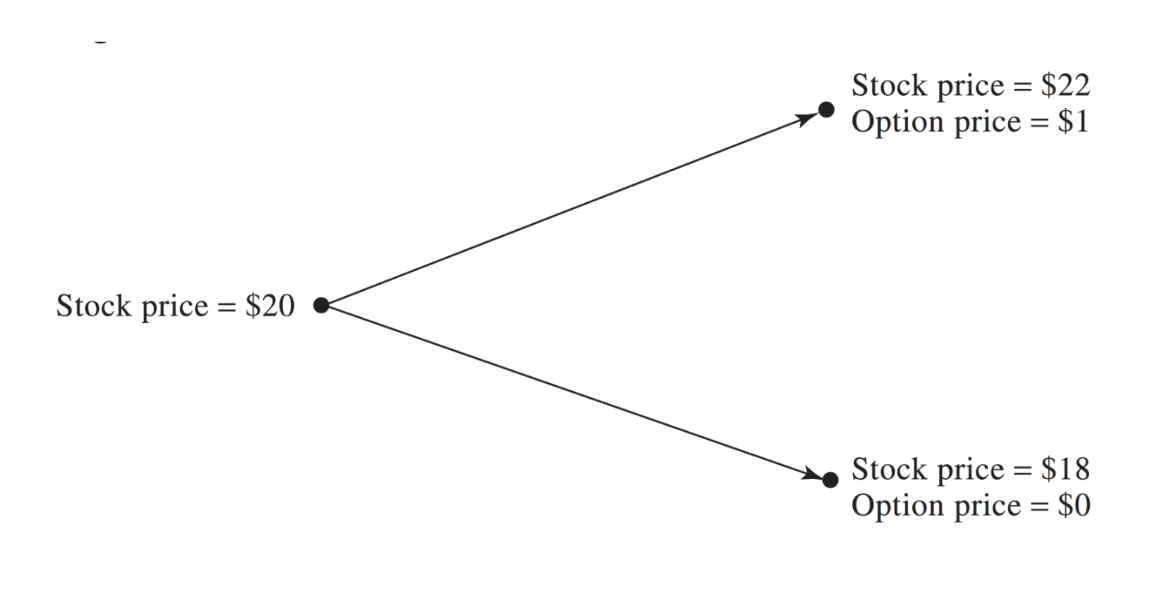
\includegraphics[scale=0.5]{tree-ex.png}

\end{figure}
\end{center}

\textbf{Solution:}

To determine the value of the European call option at time $T$, when the 

stock price can be either \$22 or \$18, we compare the option's strike price 

(\$21) with the potential stock prices.

\begin{enumerate}
    \item If the stock price at time $T$ is \$22, then exercising the call option allows the holder to buy the stock for \$21, which is less than the market price. Therefore, the option is worth \$22 - \$21 = \$1.
    \item If the stock price at time $T$ is \$18, then exercising the call option would result in buying the stock for \$21, which is more than the market price. In this case, it's not economically beneficial to exercise the option, so its value is \$0.
\end{enumerate}

So, at time $T$, the value of the option is either \$1 or \$0, depending on whether 

the stock price is \$22 or \$18 respectively.

\subsection*{Exercise 59}
\textbf{Question:} Show that if $S_T$ = 22, then the total value of the portfolio at time T is 22$\Delta$ - 1

\textbf{Solution:}

In this case the owner of the portfolio will exercise the right to buy the stock 

since the strike price is lower than the present value. Exercising this at time 

T the portfolio will now be $\Delta$ shares valued at \$22 and minus \$1 as a result 

of being in one short position of the call option.


\subsection*{Exercise 60}
\textbf{Question:} Show that if $S_T$ = 18, then the total value of the portfolio at time T is 18$\Delta$ 

\textbf{Solution:}

In this case none of the options will be exercised so at time T the portfolio 

will now be $\Delta$ shares valued at \$18 each.

\subsection*{Exercise 61}
\textbf{Question:} Find the value of $\Delta$ that makes this portfolio riskless, and conclude that, regardless of whether the stock price moves up or down, the value of the portfolio is always \$4.5 at time T  

\textbf{Solution:}

Leveraging exercises 60 and 59 we get,

22$\Delta$ - 1 = 4.5 and 18$\Delta$ = 4.5

$\implies$ 40$\Delta$ = 10 

$\therefore$ $\Delta$ = .25

\subsection*{Exercise 62}
\textbf{Question:} Suppose that the risk-free annual interest rate (compounded continuously) is 12\% and that T = 3 months. Show that the value of the portfolio today is \$4.367.

\textbf{Solution:}
Assuming that $\Delta = .25$, the future value is guaranteed to be 4.5.

$\implies$ present value = $4.5e^{-(.12/12) \cdot 3}$

$\therefore$ present value = \$4.367.

\subsection*{Exercise 63}
\textbf{Question:} Show that, in the absence of arbitrage, the price of the call option today is \$0.633.

\textbf{Solution:}

Leveraging exercise 62,

\$4.367 = \$.25 * 20 - (Price of Call Option)

$\implies$ \$4.367 - \$.25 * 20  = -(Price of Call Option)

$\implies$ -0.367 = -(Price of Call Option)

$\therefore$ Price of Call Option = \$0.633


\subsection*{Exercise 64}
\textbf{Question:} Recall that the portfolio is riskless if the portfolio is worth the same amount at time T in both
cases (i.e. $S_T$ = $S_{0}u$ or $S_T$ = $S_{0}d$). Find the value of $\Delta$ that makes the portfolio riskless.

\textbf{Solution:}

$\Delta S_{0}u - f_u = \Delta S_{0}d - f_d$

$\therefore$ $\Delta$ = $\frac{f_u - f_d}{S_0(u - d)}$

\subsection*{Exercise 65}
\textbf{Question:} Use the present value of the portfolio and the expression for $\Delta$ that you obtained in the previous exercise to show that, $$f=e^{-rT}\left[pf_u+(1-p)f_d\right],$$ where $$p=\frac{e^{rT}-d}{u-d}.$$

\textbf{Solution:}

Generalizing Exercise 63 we get the present value of the option (f) to be,

\vspace{\baselineskip}

f = $\Delta$ $S_0$ - (present value of portfolio)

\vspace{\baselineskip}

$\implies$ f = ($\frac{f_u - f_d}{u - d}$) - ($e^{-rt}$ [$\frac{f_u - f_d}{u - d}$$d - f_d$])

\vspace{\baselineskip}

$\implies$ f = $e^{-rt}$[$\frac{f_{u}e^{rt}}{u-d}$ - $\frac{f_{d}e^{rt}}{u-d}$ - $\frac{f_{u}d}{u-d}$ + $\frac{f_{d}u}{u-d}$ + $\frac{f_{d}d}{u-d}$ - $\frac{f_{d}d}{u-d}$]

\vspace{\baselineskip}

$\implies$ f = $e^{-rt}$[$\frac{e^{rt} - d}{u-d}$$f_u$ - $\frac{u - e^{rt}}{u-d}$$f_d$]

\vspace{\baselineskip}

Now after setting $p$ = $\frac{e^{rT}-d}{u-d}$ we conclude that,

\vspace{\baselineskip}

$\therefore$ f = $e^{-rT}\left[pf_u+(1-p)f_d\right]$

\subsection*{Exercise 66}
\textbf{Question:} Use this expression for f to show that f = \$0.633 for the numerical example considered previously in this section.

\textbf{Solution:}

\$0.633 = $e^{-\left(\frac{0.12}{12}\cdot3\right)} \cdot \left(\frac{e^{\left(\frac{0.12}{12}\cdot3\right)} - \frac{18}{20}}{\frac{22}{20} - \frac{18}{20}} \cdot 1 + \left(1 - \frac{e^{\left(\frac{0.12}{12}\cdot3\right)} - \frac{18}{20}}{\frac{22}{20} - \frac{18}{20}}\right) \cdot 0\right)$

\subsection*{Exercise 67}
\textbf{Question:} A stock price is currently \$100. Over each of the next two 6-month periods it is expected to go up
by 10\% or down by 10\%. The risk-free interest rate is 8\% per annum with continuous compounding. What is the
value of a 1-year European call option with a strike price of \$100

\textbf{Solution:}

\$9.61 = $e^{-2\left(.5\cdot.08\right)}\cdot\left(\left(\frac{e^{\left(.5\cdot.08\right)}-\frac{90}{100}}{\frac{110}{100\ }-\frac{90}{100}}\right)^{2}\cdot21\ +\ \left(1-\left(\frac{e^{\left(.5\cdot.08\right)}-\frac{90}{100}}{\frac{110}{100\ }-\frac{90}{100}}\right)^{2}\right)\cdot0\right))$


\subsection*{Exercise 68}
\textbf{Question:} For the situation considered in the previous exercise, what is the value of a 1-year European put option with a strike price of \$100?

\textbf{Solution:}

Using put call parity c + $Ke^{-rt}$ = p + $S_0$,

$\implies$ 9.61 + $100e^{-.08 \cdot 1}$ = p + \$100

$\therefore$ p = 9.61 + $100e^{-.08 \cdot 1}$ - \$100 = \$1.92

\subsection*{Exercise 69}
\textbf{Question:} A stock price is currently \$25. It is known that at the end of 2 months it will be either \$23 or \$27.
The risk-free interest rate is 10\% per annum with continuous compounding. Suppose $S_T$ is the stock price at the
end of 2 months. What is the value of a derivative that pays $S_T^{2}$ at this time?

\textbf{Solution:}

If after two months, the price could either be \$23 (making the value of the 

option $23^2 = 529$) or \$27 (making the value of the option $27^2 = 729$), 

consider the portfolio to have $\Delta$ shares and one derivative. Then the value 

of the portfolio in two months is
\[
27\Delta - 729 \text{ or } 23\Delta - 529.
\]

\[
\implies 27\Delta - 729 = 23\Delta - 529 \implies 4\Delta = 200 \implies \Delta = 50.
\]

That means the value of portfolio is $27(50) - 729 = 621$.

This implies that the current value of the portfolio with the value of the 

option (derivative) to be $y$ and assuming $\Delta$ = \$50
\[
\implies 50 \cdot 25 - y.
\]

As it should at least earn the risk-free rate, that means the current value of 

the portfolio, earning risk-free rate should be the same as the future value 

of the portfolio = $621$.

\[
\implies (1250 - y)e^{0.10 \cdot \frac{2}{12}} = 621.
\]

\[
\implies 1250 \cdot e^{0.10 \cdot \frac{2}{12}} - y \cdot e^{0.10 \cdot \frac{2}{12}} = 621.
\]

\[
\implies y \cdot e^{0.10 \cdot \frac{2}{12}} = 1250 \cdot e^{0.10 \cdot \frac{2}{12}} - 621.
\]

\[
\therefore y = 639.3.
\]

\subsection*{Exercise 70}
\textbf{Question:} Consider a stock whose current price is $S_0$ and a European call option on the stock whose current price is $f$.  Suppose that there are two time steps, each of length $\Delta t$, before expiry, and that during each time step, the stock price either moves up to $u$ times its initial value ($u>1$) or down to $d$ times its initial value ($d<1$).  This is illustrated in the following figure, using the same notation as in the previous figure for the payoff from the option at each stage.  (For example, $f_{uu}$ is the value of the option at time $2\Delta t=T$ if $S_T=u^2S_0$, i.e. if the stock increases in value at each time step.

\begin{center}
\begin{figure}[h]
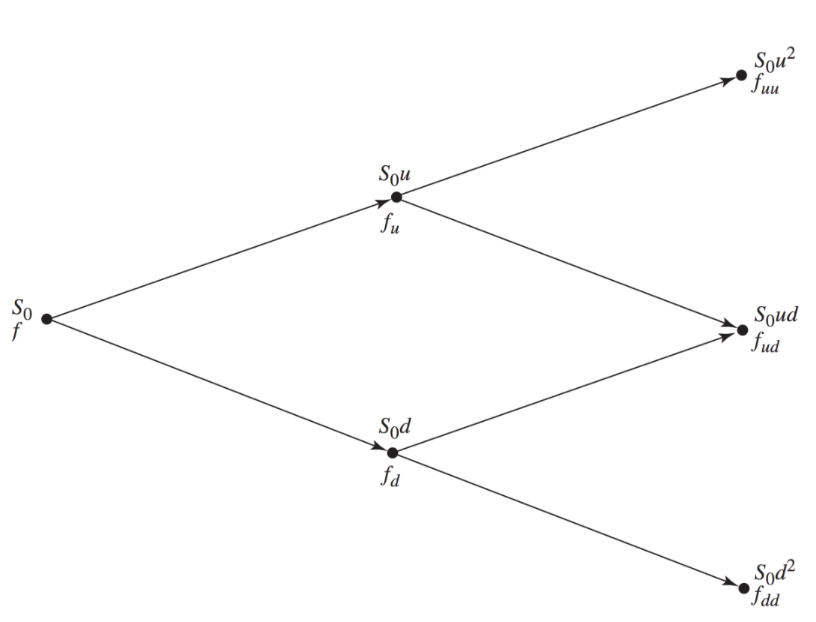
\includegraphics[scale=0.7]{p1.png}
\end{figure}
\end{center}
Show that
f = $e^{-2r \Delta t} [p^{2}f_{uu} + 2p(1 - p)f_{ud} + (1 - p)^{2}f_{dd}]$

\textbf{Solution:}
Given the option value at time $t = 0$, $f$, is determined by:

\[ f = e^{-r \Delta t} [pf_u + (1 - p)f_d] \]

where:
\begin{itemize}
  \item $f_u$ is the value of the option at time $\Delta t$ if the stock price increases to $uS_0$.
  \item $f_d$ is the value of the option at time $\Delta t$ if the stock price decreases to $dS_0$.
  \item $p$ is the risk-neutral probability of an up movement, and $1 - p$ is the probability of a down movement.
  \item $r$ is the risk-free interest rate.
\end{itemize}

We can apply this formula at time $\Delta t$ again to find $f_u$ and $f_d$:

\[ f_u = e^{-r \Delta t} [pf_{uu} + (1 - p)f_{ud}] \]
\[ f_d = e^{-r \Delta t} [pf_{ud} + (1 - p)f_{dd}] \]

Substituting these expressions back into the formula for $f$, we get:

\[ f = e^{-r \Delta t} [p(e^{-r \Delta t} [pf_{uu} + (1 - p)f_{ud}]) + (1 - p)(e^{-r \Delta t} [pf_{ud} + (1 - p)f_{dd}])] \]

Simplifying this expression, we obtain:

\[ f = e^{-2r \Delta t} [p^{2}f_{uu} + 2p(1 - p)f_{ud} + (1 - p)^{2}f_{dd}] \]

Which is the desired result.

\subsection*{Exercise 71}
\textbf{Question:} A stock price is currently \$50. Over each of the next two 3-month periods it is expected to go up by 6\% or down by 5\%. The risk-free interest rate is 5\% per annum with continuous compounding. What is the value of a 6-month European call option with a strike price of \$51?

\textbf{Solution:}

\$1.635 = $e^{-\left(2\cdot\frac{.05}{12}\cdot3\right)}\cdot\left(\left(\frac{e^{\left(\frac{.05}{12}\cdot3\right)}-.95}{1.06-.95}\right)^{2}\cdot5.18\right)$

Since $f_{ud}$ and $f_{dd}$ both equal to 0.

\subsection*{Exercise 72}

Let \( S_n \) be the number of successes in \( n \) Bernoulli trials with probability \( p \) of success on each trial. We want to show that
\[
E[S_n] = np.
\]

\textbf{Solution}

Consider the random variable \( S_n \), which represents the number of successes 

in \( n \) independent Bernoulli trials. We can write \( S_n \) as the sum of \( n \) 

independent Bernoulli random variables \( X_i \), where \( X_i = 1 \) if the \( i \)-th trial is 

a success, and \( X_i = 0 \) otherwise. Therefore,
\[
S_n = \sum_{i=1}^n X_i.
\]

To find \( E[S_n] \), we use the linearity of expectation:
\[
E[S_n] = E\left[ \sum_{i=1}^n X_i \right] = \sum_{i=1}^n E[X_i].
\]

Since each \( X_i \) is a Bernoulli random variable with parameter \( p \), the expected 

value of \( X_i \) is:
\[
E[X_i] = 1 \cdot p + 0 \cdot (1-p) = p.
\]

Substituting \( E[X_i] = p \) into the sum, we get:
\[
E[S_n] = \sum_{i=1}^n E[X_i] = \sum_{i=1}^n p = np.
\]

Therefore, we have shown that
\[
E[S_n] = np.
\]

\subsection*{Exercise 73}

Let \(X\) be a numerically-valued discrete random variable with expected value \(\mu = E[X]\). We want to show that
\[
V(X) = E[X^2] - \mu^2.
\]

\textbf{Solution}

The variance of \(X\), denoted by \(V(X)\), is defined as:
\[
V(X) = E[(X - \mu)^2].
\]

We can expand the expression inside the expectation:
\[
(X - \mu)^2 = X^2 - 2X\mu + \mu^2.
\]

Using the linearity of expectation, we take the expectation of both sides:
\[
E[(X - \mu)^2] = E[X^2 - 2X\mu + \mu^2].
\]

Since expectation is a linear operator, we can separate the terms:
\[
E[X^2 - 2X\mu + \mu^2] = E[X^2] - E[2X\mu] + E[\mu^2].
\]

Next, we use the fact that \(\mu\) is a constant and can be taken out of the 

expectation:
\[
E[2X\mu] = 2\mu E[X].
\]

Since \(E[X] = \mu\), we have:
\[
E[2X\mu] = 2\mu \cdot \mu = 2\mu^2.
\]

Also, \(E[\mu^2]\) is simply \(\mu^2\) because \(\mu^2\) is a constant:
\[
E[\mu^2] = \mu^2.
\]

Combining these results, we get:
\[
E[X^2 - 2X\mu + \mu^2] = E[X^2] - 2\mu^2 + \mu^2.
\]

Simplifying the right-hand side:
\[
E[X^2] - 2\mu^2 + \mu^2 = E[X^2] - \mu^2.
\]

Therefore, we have shown that the variance \(V(X)\) is:
\[
V(X) = E[X^2] - \mu^2.
\]

\subsection*{Exercise 74}

Let \( S_n \) be the number of successes in \( n \) Bernoulli trials with probability \( p \) of success on each trial, and let \( q = 1 - p \). We want to show that
\[
V[S_n] = \sigma^2 = npq.
\]

\textbf{Solution}

Consider the random variable \( S_n \), which represents the number of successes 

in \( n \) 

independent Bernoulli trials. We can write \( S_n \) as the sum of \( n \) independent 

Bernoulli random variables \( X_i \), where \( X_i = 1 \) if the \( i \)-th trial is a success, 

and \( X_i = 0 \) otherwise. Therefore,
\[
S_n = \sum_{i=1}^n X_i.
\]

To find \( V[S_n] \), we use the properties of variance. The variance 

of the sum of independent random variables is the sum of their variances:
\[
V[S_n] = V\left( \sum_{i=1}^n X_i \right) = \sum_{i=1}^n V(X_i).
\]

Since each \( X_i \) is a Bernoulli random variable with parameter \( p \), the variance 

of \( X_i \) is given by:
\[
V(X_i) = p(1 - p) = pq.
\]

Substituting \( V(X_i) = pq \) into the sum, we get:
\[
V[S_n] = \sum_{i=1}^n V(X_i) = \sum_{i=1}^n pq = npq.
\]

Therefore, we have shown that
\[
V[S_n] = npq.
\]

\subsection*{Exercise 75}

Show that for any \( x \),
\[
1 - N(x) = N(-x),
\]
i.e., the probability that a random draw from the standard normal distribution is above \( x \), \( 1 - N(x) \), equals the probability that the draw is below \( -x \), \( N(-x) \).

\textbf{Solution}

Let \( X \) be a random variable that follows the standard normal distribution, 

i.e., \( X \sim N(0, 1) \).

\vspace{\baselineskip}

The cumulative distribution function (CDF) of the standard normal 

distribution, \( N(x) \), is given by:
\[
N(x) = P(X \leq x).
\]

We need to show that:
\[
1 - N(x) = N(-x).
\]

First, recall that the standard normal distribution is symmetric about zero. 

This implies that for any \( x \):
\[
P(X \leq -x) = P(X \geq x).
\]

Next, using the definition of the CDF:
\[
N(-x) = P(X \leq -x).
\]

Because of the symmetry of the standard normal distribution, we have:
\[
P(X \leq -x) = P(X \geq x).
\]

Also, we know that:
\[
P(X \geq x) = 1 - P(X \leq x).
\]

Therefore:
\[
P(X \leq -x) = 1 - P(X \leq x).
\]

Substituting back into the CDF:
\[
N(-x) = 1 - P(X \leq x) = 1 - N(x).
\]

Thus, we have shown that:
\[
1 - N(x) = N(-x).
\]

\subsection*{Exercise 76}

Show that the price of a European put option on a non-dividend paying stock with strike price \( K \) and expiry \( T \) is
\[
p = Ke^{-rT} N(-d_2) - S_0 N(-d_1),
\]
where \( d_1 \) and \( d_2 \) are defined as follows:
\[
d_1 = \frac{\ln(S_0 / K) + (r + \sigma^2 / 2) T}{\sigma \sqrt{T}},
\]
\[
d_2 = d_1 - \sigma \sqrt{T}.
\]

\textbf{Solution:}

The Black-Scholes formula for the price of a European call option is given 

by:
\[
c = S_0 N(d_1) - Ke^{-rT} N(d_2),
\]

where \( N(x) \) is the cumulative distribution function for a standard normal 

distribution.

\vspace{\baselineskip}

To find the price of the corresponding European put option, we can use the 

put-call parity relationship for European options, which states:
\[
c - p = S_0 - Ke^{-rT}.
\]

Solving for \( p \), we get:
\[
p = c - S_0 + Ke^{-rT}.
\]

Substitute the expression for \( c \):
\[
p = \left( S_0 N(d_1) - Ke^{-rT} N(d_2) \right) - S_0 + Ke^{-rT}.
\]

Rearranging terms, we obtain:
\[
p = S_0 N(d_1) - S_0 - Ke^{-rT} N(d_2) + Ke^{-rT}.
\]

Factor out common terms:
\[
p = S_0 (N(d_1) - 1) + Ke^{-rT} (1 - N(d_2)).
\]

Using the properties of the cumulative distribution function,

\( N(x) + N(-x) = 1 \), we have:
\[
N(-d_1) = 1 - N(d_1),
\]
\[
N(-d_2) = 1 - N(d_2).
\]

Thus, the put option price simplifies to:
\[
p = S_0 N(-d_1) - Ke^{-rT} N(-d_2).
\]

Hence, we have shown that the price of a European put option is:
\[
p = Ke^{-rT} N(-d_2) - S_0 N(-d_1).
\]

\subsection*{Exercise 77}

A non-dividend paying stock has current value $S_0$ = \$41. The volatility is $\sigma$ = 0.3 and the risk-free
interest rate is r = 8\%. Find the price of a European call option on the stock with strike price K = \$40 and
expiry T = 3 months.

\textbf{Solution:}

c = $41\cdot N\left(d_{1}\right)-40e^{-\left(.08\cdot3\right)}\cdot N\left(d_{2}\right)$

\vspace{\baselineskip}

with,

\vspace{\baselineskip}

$d_{1}=\frac{\ln\left(\frac{41}{40}\right)+\left(.08+\ \frac{.3^{2}}{2}\right)3}{.3\cdot3}$

\vspace{\baselineskip}

and,

\vspace{\baselineskip}

$d_{2} =\  d_{1}\ -\ .3\cdot\sqrt{3}$

\vspace{\baselineskip}

$\therefore c = \$3.399$

\subsection*{Exercise 78}

\textbf{Solution:}

p = $40e^{-\left(.08\cdot3\right)}\cdot N\left(-d_{2}\right)-41\cdot N\left(-d_{1}\right)$

\vspace{\baselineskip}

with,

\vspace{\baselineskip}

$d_{1}=\frac{\ln\left(\frac{41}{40}\right)+\left(.08+\ \frac{.3^{2}}{2}\right)3}{.3\cdot3}$

\vspace{\baselineskip}

and,

\vspace{\baselineskip}

$d_{2} =\  d_{1}\ -\ .3\cdot\sqrt{3}$

\vspace{\baselineskip}

$\therefore p = \$1.607$

\subsection*{Exercise 79}
Find the binomial approximation for the call option in Exercise 77 with \( n = 1, n = 2, n = 10, n = 12, \) and \( n = 100 \). What happens to the approximation as \( n \) increases? Where the call option \( c = e^{-rT} \sum_{j=0}^{n} \binom{n}{j} p^j (1-p)^{n-j} \max(S_0 u^j d^{n-j} - K, 0) \).

\textbf{Solution:}

To find the binomial approximation for the call option, we use the binomial pricing model. We first need to determine the up and down factors, \( u \) and \( d \), and the risk-neutral probability \( p \).

Given:
\[
S_0 = \$41, \quad \sigma = 0.3, \quad r = 0.08, \quad K = \$40, \quad T = \frac{3}{12} \text{ years}
\]

The up and down factors are given by:
\[
u = e^{\sigma \sqrt{\frac{T}{n}}}, \quad d = e^{-\sigma \sqrt{\frac{T}{n}}}
\]

The risk-neutral probability \( p \) is given by:
\[
p = \frac{e^{r \frac{T}{n}} - d}{u - d}
\]

The value of the call option is then given by:
\[
c = e^{-rT} \sum_{j=0}^{n} \binom{n}{j} p^j (1-p)^{n-j} \max(S_0 u^j d^{n-j} - K, 0)
\]

We now compute the binomial approximation for different values of \( n \):

\textbf{For \( n = 1 \):}
\[
u = e^{0.3 \sqrt{\frac{3}{12}}}, \quad d = e^{-0.3 \sqrt{\frac{3}{12}}}
\]
\[
p = \frac{e^{0.08 \frac{3}{12}} - d}{u - d}
\]

\[
3.96396 = e^{-0.08 \cdot \frac{3}{12}} \left[ p \max(S_0 u - K, 0) + (1 - p) \max(S_0 d - K, 0) \right]
\]

\textbf{For \( n = 2 \):}
\[
3.33095 = e^{0.3 \sqrt{\frac{3}{24}}}, \quad d = e^{-0.3 \sqrt{\frac{3}{24}}}
\]
\[
p = \frac{e^{0.08 \frac{3}{24}} - d}{u - d}
\]

\[
3.33095 = e^{-0.08 \cdot \frac{3}{12}} \sum_{j=0}^{2} \binom{2}{j} p^j (1-p)^{2-j} \max(S_0 u^j d^{2-j} - K, 0)
\]

\textbf{For \( n = 10 \):}
\[
u = e^{0.3 \sqrt{\frac{3}{120}}}, \quad d = e^{-0.3 \sqrt{\frac{3}{120}}}
\]
\[
p = \frac{e^{0.08 \frac{3}{120}} - d}{u - d}
\]

\[
3.42679 = e^{-0.08 \cdot \frac{3}{12}} \sum_{j=0}^{10} \binom{10}{j} p^j (1-p)^{10-j} \max(S_0 u^j d^{10-j} - K, 0)
\]

\textbf{For \( n = 12 \):}
\[
u = e^{0.3 \sqrt{\frac{3}{144}}}, \quad d = e^{-0.3 \sqrt{\frac{3}{144}}}
\]
\[
p = \frac{e^{0.08 \frac{3}{144}} - d}{u - d}
\]

\[
3.42677 = e^{-0.08 \cdot \frac{3}{12}} \sum_{j=0}^{12} \binom{12}{j} p^j (1-p)^{12-j} \max(S_0 u^j d^{12-j} - K, 0)
\]

\textbf{For \( n = 100 \):}
\[
u = e^{0.3 \sqrt{\frac{3}{1200}}}, \quad d = e^{-0.3 \sqrt{\frac{3}{1200}}}
\]
\[
p = \frac{e^{0.08 \frac{3}{1200}} - d}{u - d}
\]

\[
3.4003 = e^{-0.08 \cdot \frac{3}{12}} \sum_{j=0}^{100} \binom{100}{j} p^j (1-p)^{100-j} \max(S_0 u^j d^{100-j} - K, 0)
\]

As \( n \) increases, the binomial approximation converges to the Black-Scholes value. 

\subsection*{Exercise 80}

A non-dividend paying stock has current value \( S_0 = \$120 \). The volatility is \( \sigma = 0.3 \) and the risk-free interest rate is \( r = 8\% \). (i) Find the price of a European call option on the stock with strike price \( K = \$100 \) and expiry \( T = 1 \) year. (ii) Compute the price of the European call option for several values of large \( T \). What happens to the price of the European call option as \( T \to \infty \)?

\vspace{\baselineskip}

\textbf{Solution:}

\vspace{\baselineskip}

(i)

The price of a European call option is given by the Black-Scholes formula:

\[
c = S_0 N(d_1) - Ke^{-rT} N(d_2)
\]

where,

\[
d_1 = \frac{\ln\left(\frac{S_0}{K}\right) + \left(r + \frac{\sigma^2}{2}\right)T}{\sigma \sqrt{T}}
\]

\[
d_2 = d_1 - \sigma \sqrt{T}
\]

Given the parameters:
\[
S_0 = 120, \quad K = 100, \quad \sigma = 0.3, \quad r = 0.08, \quad T = 1
\]

First, compute \( d_1 \):

\[
d_1 = \frac{\ln\left(\frac{120}{100}\right) + \left(0.08 + \frac{0.3^2}{2}\right) \cdot 1}{0.3 \sqrt{1}} = \frac{\ln(1.2) + 0.08 + 0.045}{0.3} = \frac{0.1823 + 0.125}{0.3} = \frac{0.3073}{0.3} \approx 1.0243
\]

Then compute \( d_2 \):

\[
d_2 = d_1 - 0.3 \sqrt{1} = 1.0243 - 0.3 = 0.7243
\]

Using the cumulative distribution function of the standard normal 

distribution, \( N(d_1) \) and \( N(d_2) \):

\[
N(d_1) \approx 0.8475, \quad N(d_2) \approx 0.7656
\]

Now, compute the call price \( c \):

\[
c = 120 \cdot 0.8475 - 100 e^{-0.08 \cdot 1} \cdot 0.7656 = 120 \cdot 0.8475 - 100 \cdot 0.9231 \cdot 0.7656 \approx 101.70 - 70.65 \approx 31.05
\]

Therefore, the price of the European call option is \( \boxed{\$31.05} \).

\vspace{\baselineskip}

(ii) 


As \( T \) increases, the terms in the Black-Scholes formula change. 

For very large \( T \), the behavior of \( d_1 \) and \( d_2 \) is dominated by \( T \).

\[
d_1 = \frac{\ln\left(\frac{S_0}{K}\right) + \left(r + \frac{\sigma^2}{2}\right)T}{\sigma \sqrt{T}}
\]

\[
d_2 = d_1 - \sigma \sqrt{T} = \frac{\ln\left(\frac{S_0}{K}\right) + \left(r + \frac{\sigma^2}{2}\right)T}{\sigma \sqrt{T}} - \sigma \sqrt{T}
\]

For large \( T \):

\[
d_1 \approx \frac{(r + \frac{\sigma^2}{2})T}{\sigma \sqrt{T}} = \frac{(r + \frac{\sigma^2}{2})\sqrt{T}}{\sigma}
\]

\[
d_2 \approx \frac{(r + \frac{\sigma^2}{2})\sqrt{T}}{\sigma} - \sigma \sqrt{T} = \left(\frac{r + \frac{\sigma^2}{2}}{\sigma} - \sigma\right) \sqrt{T}
\]

Since \( \frac{r + \frac{\sigma^2}{2}}{\sigma} - \sigma \) is a constant, as \( T \to \infty \), \( d_1 \) and \( d_2 \) increase indefinitely. 

\vspace{\baselineskip}

Consequently, \( N(d_1) \) and \( N(d_2) \) approach 1.

\vspace{\baselineskip}

Therefore, the price of the call option approximates:

\[
c \approx S_0 - K e^{-rT}
\]

As \( T \to \infty \), \( e^{-rT} \to 0 \), so:

\[
c \approx S_0
\]

Hence, the price of the European call option approaches \( S_0 = \$120 \) as 

\( T \to \infty \).

\subsection*{Exercise 81}

Consider a bull spread in which you buy a 40-strike call and sell a 45-strike call. Suppose \( S_0 = \$40 \), \( \sigma = 0.30 \), \( r = 0.08 \), and \( T = 0.5 \).

\vspace{\baselineskip}

\noindent Draw a graph with stock prices ranging from \$20 to \$60 depicting the profit 

on the bull spread at expiry.

\textbf{Solution:}

To draw the profit graph of a bull spread at expiry, we need to consider the 

payoff of the long call (strike price \( K_1 = 40 \)) and the short call 

(strike price \( K_2 = 45 \)).

\vspace{\baselineskip}

The payoff of a long call option is:
\[
\max(S_T - K_1, 0)
\]

The payoff of a short call option is:
\[
-\max(S_T - K_2, 0)
\]

The payoff of the bull spread is the difference between these two payoffs:
\[
\text{Payoff} = \max(S_T - 40, 0) - \max(S_T - 45, 0)
\]

To calculate the profit, we subtract the net premium paid for the spread.

\vspace{\baselineskip}

To find the premium for both options, we will compute their Black-Scholes 

values:

\[
c_{40} = S_0 N(d_{1,40}) - K_1 e^{-rT} N(d_{2,40})
\]

with,

\[
d_{1,40} = \frac{\ln\left(\frac{S_0}{K_1}\right) + \left(0.08 + \frac{0.3^2}{2}\right) \cdot 0.5}{0.3 \sqrt{0.5}}
\]

\[
d_{2,40} = d_{1,40} - 0.3 \sqrt{0.5}
\]

Similarly,

\[
c_{45} = S_0 N(d_{1,45}) - K_2 e^{-rT} N(d_{2,45})
\]

with,

\[
d_{1,45} = \frac{\ln\left(\frac{S_0}{K_2}\right) + \left(0.08 + \frac{0.3^2}{2}\right) \cdot 0.5}{0.3 \sqrt{0.5}}
\]

\[
d_{2,45} = d_{1,45} - 0.3 \sqrt{0.5}
\]

Calculating \( d_{1,40} \) and \( d_{2,40} \):

\[
d_{1,40} = \frac{\ln\left(\frac{40}{40}\right) + \left(0.08 + \frac{0.3^2}{2}\right) \cdot 0.5}{0.3 \sqrt{0.5}} = \frac{0 + \left(0.08 + 0.045\right) \cdot 0.5}{0.3 \sqrt{0.5}} = \frac{0.0625}{0.2121} \approx 0.2946
\]

\[
d_{2,40} = d_{1,40} - 0.3 \sqrt{0.5} = 0.2946 - 0.2121 \approx 0.0825
\]

Calculating \( d_{1,45} \) and \( d_{2,45} \):

\[
d_{1,45} = \frac{\ln\left(\frac{40}{45}\right) + \left(0.08 + \frac{0.3^2}{2}\right) \cdot 0.5}{0.3 \sqrt{0.5}} = \frac{\ln\left(\frac{40}{45}\right) + 0.0625}{0.2121} = \frac{-0.1178 + 0.0625}{0.2121} \approx -0.2604
\]

\[
d_{2,45} = d_{1,45} - 0.3 \sqrt{0.5} = -0.2604 - 0.2121 \approx -0.4725
\]

\vspace{\baselineskip}

Using the cumulative distribution function of the standard normal 

distribution, \( N(d_{1,40}) \approx 0.6162 \) and \( N(d_{2,40}) \approx 0.5329 \), and 

\( N(d_{1,45}) \approx 0.3978 \) and \( N(d_{2,45}) \approx 0.3181 \):

\[
c_{40} = 40 \cdot 0.6162 - 40 \cdot e^{-0.04} \cdot 0.5329 \approx 24.65 - 40 \cdot 0.9612 \cdot 0.5329 \approx 24.65 - 20.47 \approx 4.18
\]

\[
c_{45} = 40 \cdot 0.3978 - 45 \cdot e^{-0.04} \cdot 0.3181 \approx 15.91 - 45 \cdot 0.9612 \cdot 0.3181 \approx 15.91 - 13.73 \approx 2.18
\]

The net premium paid for the spread is:

\[
\text{Net Premium} = c_{40} - c_{45} \approx 4.18 - 2.18 = 2.00
\]

The profit function is then given by:

\[
\text{Profit} = \begin{cases} 
-2.00 & \text{if } S_T \leq 40 \\
S_T - 40 - 2.00 & \text{if } 40 < S_T \leq 45 \\
3.00 & \text{if } S_T > 45 
\end{cases}
\]

We now plot this using a graph.

\begin{center}
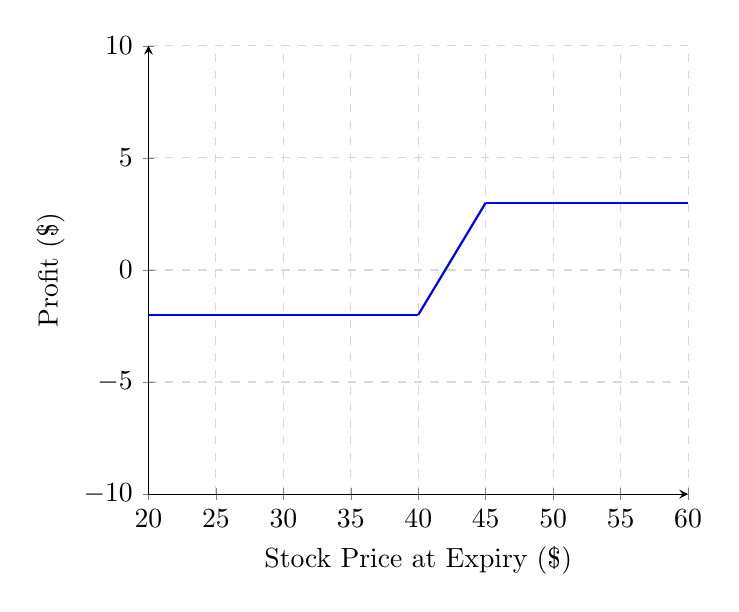
\begin{tikzpicture}
\begin{axis}[
    axis lines = left,
    xlabel = {Stock Price at Expiry (\$)},
    ylabel = {Profit (\$)},
    ymin = -10, ymax = 10,
    xmin = 20, xmax = 60,
    ytick={-10, -5, 0, 5, 10},
    xtick={20, 25, 30, 35, 40, 45, 50, 55, 60},
    grid = both,
    grid style = {dashed, gray!30}
]

\addplot[
    domain=20:40,
    samples=2,
    color=blue,
    thick
]
{-2};

\addplot[
    domain=40:45,
    samples=2,
    color=blue,
    thick
]
{x-42};

\addplot[
    domain=45:60,
    samples=2,
    color=blue,
    thick
]
{3};

\end{axis}
\end{tikzpicture}
\end{center}

The graph shows the profit of the bull spread at expiry for stock prices 

ranging from \$20 to \$60.

\subsection*{Exercise 98}
Graph the feasible region for Example 10.1.

\textbf{Solution:}
\begin{center}
    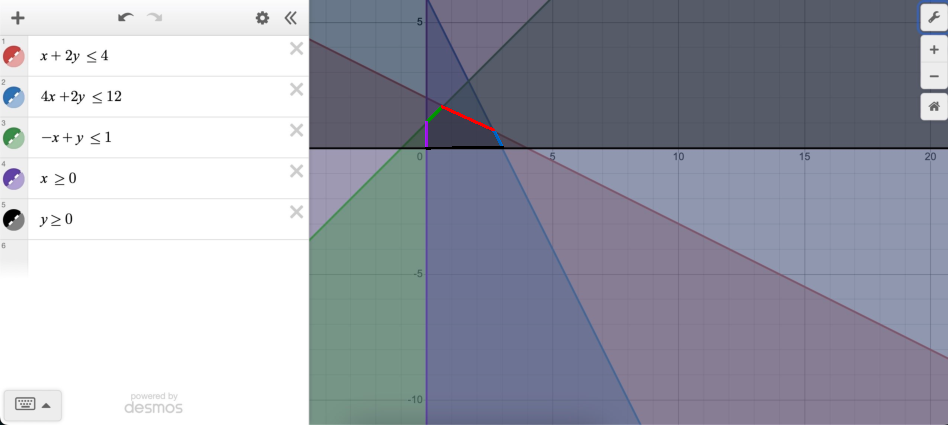
\includegraphics[width=1.2\textwidth]{Ex98.pdf}
\end{center}

The constraints are:
\[
\begin{aligned}
    x_1 + 2x_2 &\leq 4, \\
    4x_1 + 2x_2 &\leq 12, \\
    -x_1 + x_2 &\leq 1, \\
    x_1 &\geq 0, \\
    x_2 &\geq 0.
\end{aligned}
\]

\subsection*{Exercise 99}
Graph the lines \( z = x_1 + x_2 \) along with the feasible region for \( z = 0, 1, 2, 5, 15 \). Which of these represent possible values of the objective function?

\textbf{Solution:}

\begin{center}
    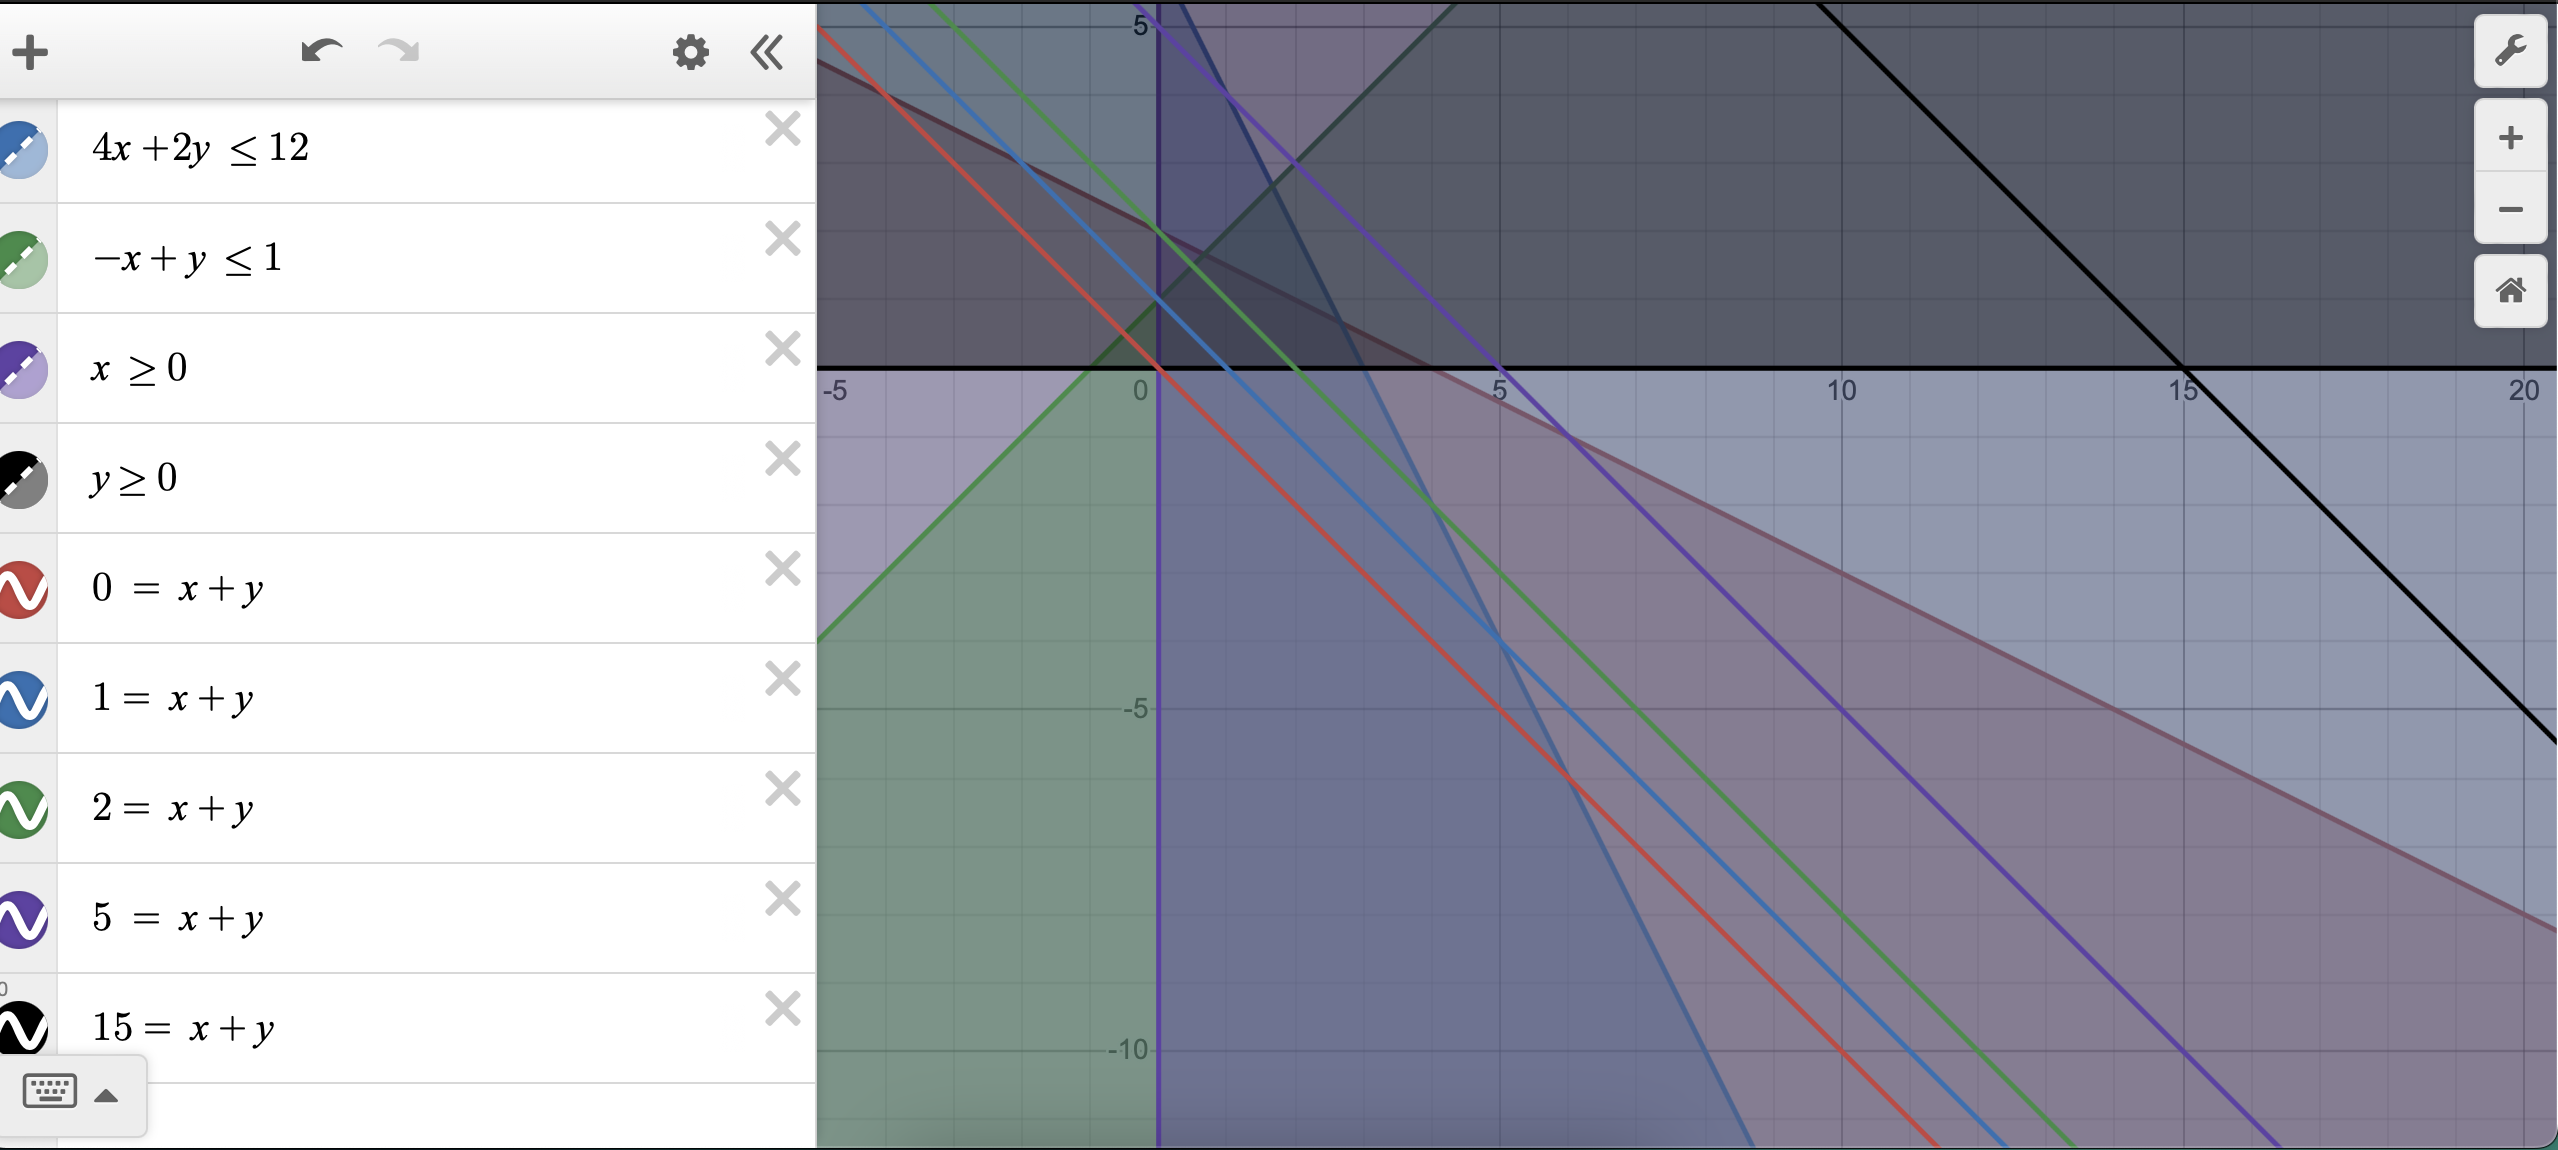
\includegraphics[width=1.2\textwidth]{Ex99.png}
\end{center}

The lines for \( z = 0, 1, 2 \) are within the feasible region. The line for \( z = 5, 15 \) 

is outside the feasible region, indicating they are not possible value for the 

objective function.

\subsection*{Exercise 100}
Find all 5 of the corner points for the feasible region of Example 10.1, and substitute each into the objective function. Verify that \( \frac{10}{3} \) is the maximum value of the objective function and that it occurs at \( (x_1, x_2) = \left( \frac{8}{3}, \frac{2}{3} \right) \).

Corner points:
\[
\begin{aligned}
    (0, 0) &\Rightarrow z = 0, \\
    (0, 2) &\Rightarrow z = 2, \\
    (2, 1) &\Rightarrow z = 3, \\
    \left( \frac{8}{3}, \frac{2}{3} \right) &\Rightarrow z = \frac{10}{3}, \\
    (3, 0) &\Rightarrow z = 3.
\end{aligned}
\]

The maximum value is \( \frac{10}{3} \), occurring at \( \left( \frac{8}{3}, \frac{2}{3} \right) \).

\subsection*{Exercise 101}
Consider the following linear programming problem: Find \( x_1 \) and \( x_2 \) to minimize \( x_1 + 3x_2 \) subject to the constraints:
\[
\begin{aligned}
    2x_1 + x_2 &\leq 10, \\
    5x_1 + 2x_2 &\geq 20, \\
    -x_1 + 2x_2 &\geq 0, \\
    x_1, x_2 &\geq 0.
\end{aligned}
\]

\begin{center}
    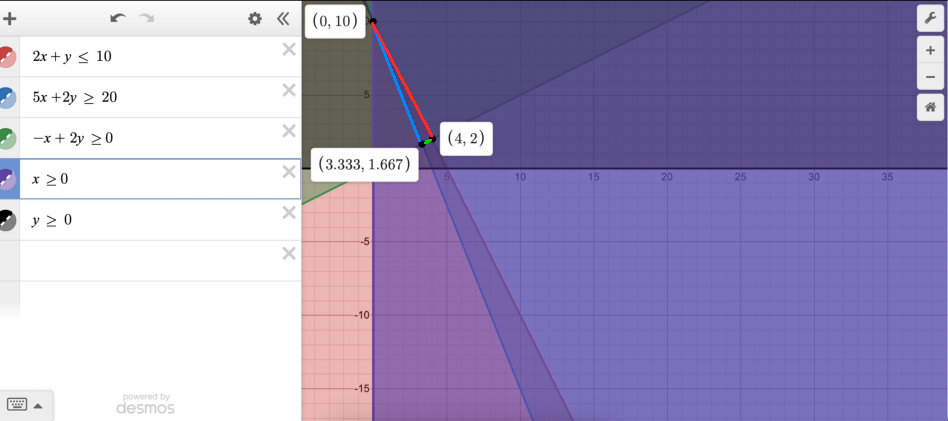
\includegraphics[width=1.2\textwidth]{Ex101.pdf}
\end{center}


\textbf{Solution}
The optimal solution is \( x_1 = \frac{10}{3} \), \( x_2 = \frac{5}{3} \) with minimum value 

\( x_1 + 3x_2 = \frac{10}{3} + \frac{15}{3} = \frac{25}{3} \).

\subsection*{Exercise 102}
Determine the range of \( \frac{c_1}{c_2} \) for which \( (x_1, x_2) = (4, 3) \) is an optimal solution of the problem:
\[
\begin{aligned}
    \text{maximize} \quad & c_1 x_1 + c_2 x_2 \\
    \text{subject to} \quad & 2x_1 + x_2 \leq 11, \\
    & -x_1 + 2x_2 \leq 2, \\
    & x_1, x_2 \geq 0.
\end{aligned}
\]

\textbf{Solution}

First we calculate the slopes of the constraints:
\[
\begin{aligned}
    \text{Slope of } 2x_1 + x_2 = 11 &\implies 2, \\
    \text{Slope of } -x_1 + 2x_2 = 2 &\implies -\frac{1}{2}.
\end{aligned}
\]

For \( (4, 3) \) to be an optimal solution, the objective function \( c_1 x_1 + c_2 x_2 \) must 

be tangent to one of these constraints at the optimal point. This means the 

slope of the objective function \( \frac{c_1}{c_2} \) must lie between the slopes of the two 

binding constraints.

\vspace{\baselineskip}

Therefore, the range of \( \frac{c_1}{c_2} \) for which \( (4, 3) \) is an optimal solution is:
\[
-\frac{1}{2} \leq \frac{c_1}{c_2} \leq 2.
\]

\subsection*{Exercise 103}

Consider the following linear programming problem, where the value of \( c_1 \) has not yet been determined. Find \( x_1 \) and \( x_2 \) to:

\[
\text{maximize} \quad c_1 x_1 + 2 x_2
\]

subject to the constraints:

\[
\begin{cases}
4x_1 + x_2 \leq 12 \\
x_1 - x_2 \geq 2 \\
x_1, x_2 \geq 0
\end{cases}
\]

Determine the optimal solutions for the various possible values of \( c_1 \) (both 

positive and negative).

\vspace{\baselineskip}

\textbf{Solution}

To solve this linear programming problem, we will consider the constraints 

and find the feasible region. We will then determine the optimal solution for 

different values of \( c_1 \).

\vspace{\baselineskip}

First, we plot the constraints:

\vspace{\baselineskip}

1. \( 4x_1 + x_2 = 12 \)
2. \( x_1 - x_2 = 2 \)

The intersection points of these lines and the feasible region will help us 

determine the optimal solution.

\vspace{\baselineskip}

Solving for the intersection of \( 4x_1 + x_2 = 12 \) and \( x_1 - x_2 = 2 \):

\vspace{\baselineskip}

1. From \( x_1 - x_2 = 2 \), we get \( x_2 = x_1 - 2 \).

2. Substitute \( x_2 = x_1 - 2 \) into \( 4x_1 + x_2 = 12 \):

\[
4x_1 + (x_1 - 2) = 12 \implies 5x_1 - 2 = 12 \implies 5x_1 = 14 \implies x_1 = \frac{14}{5}
\]

\[
x_2 = \frac{14}{5} - 2 = \frac{14}{5} - \frac{10}{5} = \frac{4}{5}
\]

So, the intersection point is \( \left( \frac{14}{5}, \frac{4}{5} \right) \).

\vspace{\baselineskip}

The vertices of the feasible region are determined by the intersection of the 

constraints with the axes and each other:

\vspace{\baselineskip}

1. Intersection of \( 4x_1 + x_2 = 12 \) with \( x_2 = 0 \):

\[
4x_1 = 12 \implies x_1 = 3 \quad \text{(Point: } (3, 0))
\]

2. Intersection of \( x_1 - x_2 = 2 \) with \( x_1 = 2 \):

\[
2 - x_2 = 2 \implies x_2 = 0 \quad \text{(Point: } (2, 0))
\]

The feasible region vertices are:

\[
(2, 0), \left( \frac{14}{5}, \frac{4}{5} \right), (3, 0)
\]


To find the optimal solution, evaluate the objective function at these vertices 

for various values of \( c_1 \).

\vspace{\baselineskip}

For \( c_1 > 0 \):
\[
\begin{aligned}
&\text{At } (2, 0): & 2c_1 \\
&\text{At } \left( \frac{14}{5}, \frac{4}{5} \right): & c_1 \cdot \frac{14}{5} + 2 \cdot \frac{4}{5} = \frac{14c_1 + 8}{5} = 2.8c_1 + 1.6 \\
&\text{At } (3, 0): & 3c_1
\end{aligned}
\]

\vspace{\baselineskip}

For \( c_1 < 0 \):
\[
\begin{aligned}
&\text{At } (2, 0): & 2c_1 \\
&\text{At } \left( \frac{14}{5}, \frac{4}{5} \right): & \frac{14c_1 + 8}{5} = 2.8c_1 + 1.6 \\
&\text{At } (3, 0): & 3c_1
\end{aligned}
\]

\vspace{\baselineskip}

Thus, the optimal solutions are:

\vspace{\baselineskip}

- For \( c_1 > 0 \), the optimal point is \( (3, 0) \) if \(c_1 > 8\), else the optimal point is 

\( (\frac{14}{5}, \frac{4}{5}) \)

\vspace{\baselineskip}

- For \( c_1 < 0 \), the optimal point is \( (2, 0) \) since \( 2c_1 \) is greater than \( 3c_1 \) and 

\( 2.8c_1 + 1.6 \).




\subsection*{Exercise 104}
A manufacturing process requires oil refineries to produce at least 2 gallons of gasoline for every gallon of fuel oil. To meet winter demand, at least 3 million gallons of fuel oil must be produced. The demand for gasoline is no more than 12 million gallons per day. It takes 0.25 hours to ship each million gallons of gasoline and 1 hour to ship each million gallons of fuel oil. No more than 6.6 hours are available for shipping. If the refinery sells gasoline for \$1.25 per gallon and fuel oil for \$1 per gallon, how much of each should be produced to maximize revenue?

\vspace{\baselineskip}

\textbf{Solution}

Let \( x_1 \) be the million gallons of gasoline and \( x_2 \) be the million gallons of fuel 

oil.

Maximize \( 1.25x_1 + x_2 \)
\[
\begin{aligned}
    2x_2 &\leq x_1, \\
    x_2 &\geq 3, \\
    x_1 &\leq 12, \\
    0.25x_1 + x_2 &\leq 6.6, \\
    x_1, x_2 &\geq 0.
\end{aligned}
\]

\textbf{Solution}:

\begin{center}
    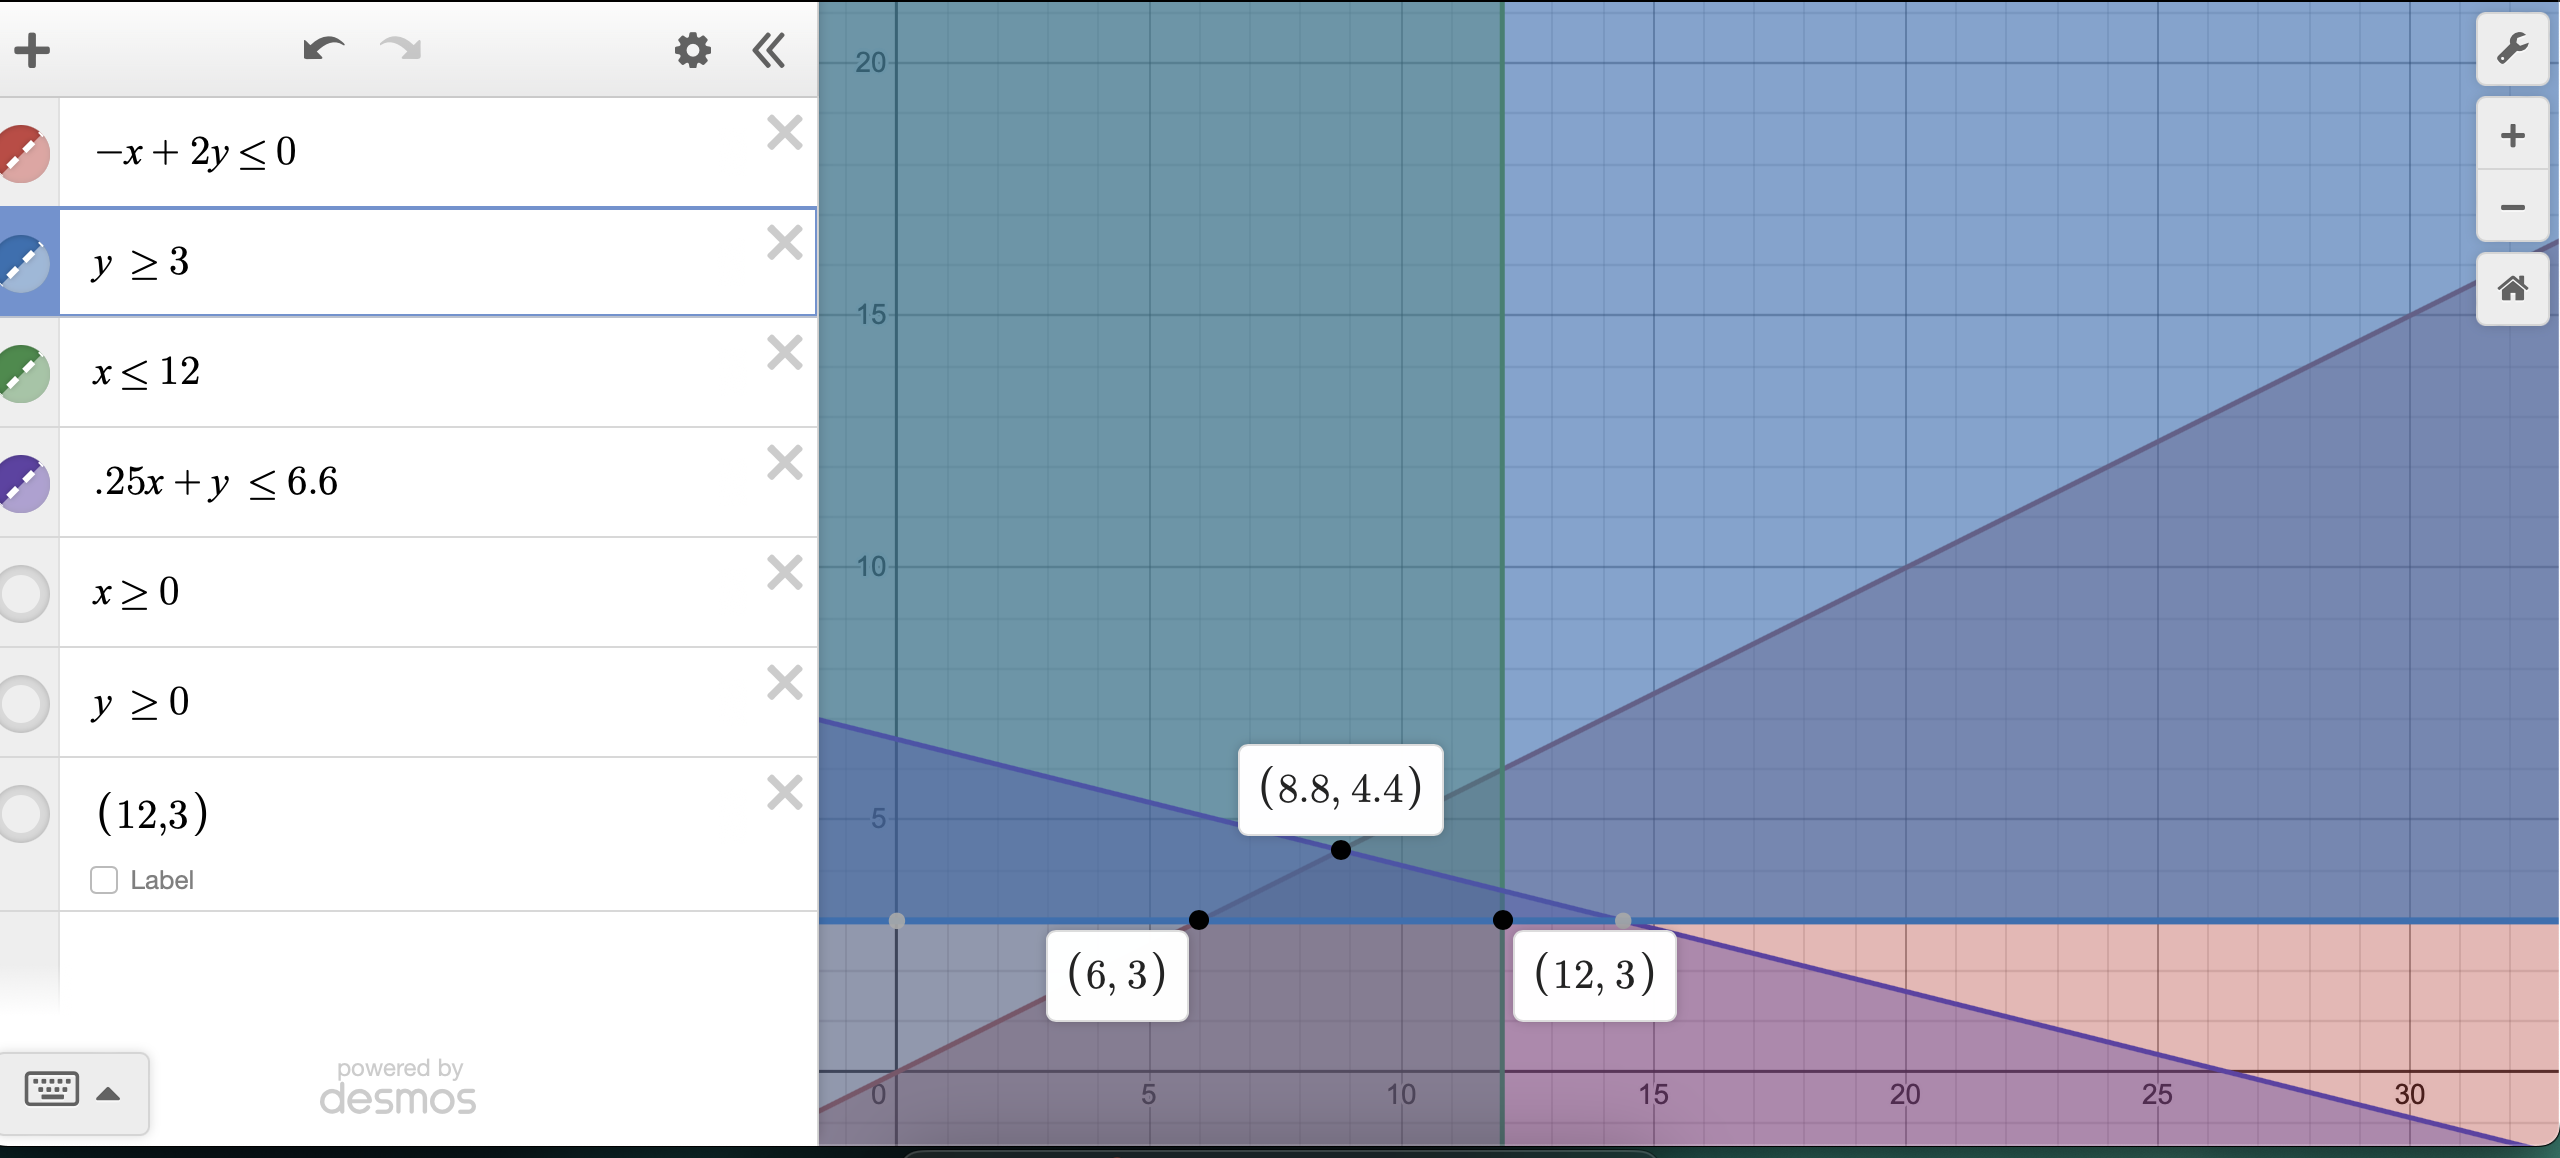
\includegraphics[width=1.2\textwidth]{Ex104.png}
\end{center}

\[
x_1 = 12, \quad x_2 = 3 \implies \\
\text{Maximum revenue} = 1.25(12) + 3 = 18
\]

\subsection*{Exercise 105}
Transform the following LP to a standard maximum problem:

\begin{align*}
\text{minimize } & \quad x_1 - 12x_2 - 2x_3 \\
\text{subject to:} & \\
5x_1 - x_2 - 2x_3 &= 10, \\
2x_1 + x_2 - 20x_3 &\geq -30, \\
x_2 &\leq 0, \\
1 &\leq x_3 \leq 4.
\end{align*}

\textbf{Solution}

To convert this to a standard maximum problem:

\vspace{\baselineskip}

1. Change the objective function to maximize by multiplying by -1:
\[
\text{maximize } -x_1 + 12x_2 + 2x_3
\]

2. Convert the inequality \(2x_1 + x_2 - 20x_3 \geq -30\) to standard form:
\[
-2x_1 - x_2 + 20x_3 \leq 30
\]

3. Convert the upper and lower bounds to standard form using new variables:
\[
w_2 = -x_2, \quad x_2 = -w_2 \Rightarrow w_2 \geq 0
\]
\[
x_3 = 1 + w_3, \quad w_3 \geq 0
\]
\[
x_3 = 4 - w_4, \quad w_4 \geq 0
\]

The transformed problem is:
\[
\text{maximize } -x_1 - 12w_2 + 2 + 2w_3
\]
subject to:
\begin{align*}
5x_1 + w_2 - 2(1 + w_3) &= 10, \\
-2x_1 - w_2 + 20(1 + w_3) &\leq 30, \\
w_2 &\geq 0, \\
w_3 &\geq 0, \\
w_4 &\geq 0.
\end{align*}

In matrix form:
\[
\text{maximize } -x_1 - 12w_2 + 2 + 2w_3
\]
subject to:
\[
\begin{bmatrix}
5 & 1 & -2 & 0 & 0 \\
-2 & -1 & 20 & 0 & 0
\end{bmatrix}
\begin{bmatrix}
x_1 \\
w_2 \\
w_3 \\
\end{bmatrix}
\leq
\begin{bmatrix}
12 \\
10
\end{bmatrix}
\]

\newpage

\subsection*{Exercises 106-110}

Given the following linear system and objective function, find the optimal solution.

\begin{equation*}
\max \{ 2x_1 + 3x_2 + x_3 \}
\end{equation*}

\[
\left\{
\begin{array}{l}
x_1 + x_2 + 4x_3 \leq 100 \\
x_1 + 2x_2 + x_3 \leq 150 \\
3x_1 + 2x_2 + x_3 \leq 320 \\
\end{array}
\right.
\]

\textbf{Solution}

Add slack variables to turn all inequalities to equalities (Exercise 106).

\[
\left\{
\begin{array}{l}
x_1 + x_2 + 4x_3 + s_1 = 100 \\
x_1 + 2x_2 + x_3 + s_2 = 150 \\
3x_1 + 2x_2 + x_3 + s_3 = 320 \\
\end{array}
\right.
\]

Create the initial tableau of the new linear system.

\[
\begin{bmatrix}
\begin{array}{cccccc|c}
x_1 & x_2 & x_3 & s_1 & s_2 & s_3 & b \\
\hline
1 & 1 & 4 & 1 & 0 & 0 & 100 \\
1 & 2 & 1 & 0 & 1 & 0 & 150 \\
3 & 2 & 1 & 0 & 0 & 1 & 320 \\
\hline
-2 & -3 & -1 & 0 & 0 & 0 & 0 \\
\end{array}
\end{bmatrix}
\begin{array}{c}
\\
s_1 \\
s_2 \\
s_3 \\
\\
\end{array}
\]

There are negative elements in the bottom row, so the current solution is 

not optimal. Thus, pivot to improve the current solution. The entering 

variable is \(x_2\) and the departing variable is \(s_2\).

\vspace{\baselineskip}

Perform elementary row operations until the pivot element is 1 and 

all other elements in the entering column are 0 (Exercise 107/108).

\[
\begin{bmatrix}
\begin{array}{cccccc|c}
x_1 & x_2 & x_3 & s_1 & s_2 & s_3 & b \\
\hline
1/2 & 0 & 7/2 & 1 & -1/2 & 0 & 25 \\
1/2 & 1 & 1/2 & 0 & 1/2 & 0 & 75 \\
2 & 0 & 0 & 0 & -1 & 1 & 170 \\
\hline
-1/2 & 0 & 1/2 & 0 & 3/2 & 0 & 225 \\
\end{array}
\end{bmatrix}
\begin{array}{c}
\\
s_1 \\
x_2 \\
s_3 \\
\\
\end{array}
\]

There are negative elements in the bottom row, so the current solution is 

not optimal. Thus, pivot to improve the current solution. The entering 

variable is \(x_1\) and the departing variable is \(s_1\).

\vspace{\baselineskip}

Perform elementary row operations until the pivot element is 1 and all other 

elements in the entering column are 0 (Exercise 109).

\[
\begin{bmatrix}
\begin{array}{cccccc|c}
x_1 & x_2 & x_3 & s_1 & s_2 & s_3 & b \\
\hline
1 & 0 & 7 & 2 & -1 & 0 & 50 \\
0 & 1 & -3 & -1 & 1 & 0 & 50 \\
0 & 0 & -14 & -4 & 1 & 1 & 70 \\
\hline
0 & 0 & 4 & 1 & 1 & 0 & 250 \\
\end{array}
\end{bmatrix}
\begin{array}{c}
\\
x_1 \\
x_2 \\
s_3 \\
\\
\end{array}
\]

There are no negative elements in the bottom row, so we know the solution 

is optimal. Thus, the solution is (Exercise 110):

\begin{equation*}
s_1 = 0, \, s_2 = 0, \, s_3 = 70, \, x_1 = 50, \, x_2 = 50, \, x_3 = 0, \, z = 250
\end{equation*}


\subsection*{Exercise 111}
An office manager needs to purchase new filing cabinets. She knows that Ace cabinets cost \$40 each, require 6 square feet of floor space, and hold 8 cubic feet of files. On the other hand, each Excello cabinet
costs \$80, requires 8 square feet of floor space, and holds 12 cubic feet. The budget permits her to spend no more than \$560, while the office has room for no more than 72 square feet of cabinets. The manager desires the greatest storage capacity within the limitations imposed by funds and space. How many of each type of cabinet should she buy?

\textbf{Solution:}

\vspace{\baselineskip}

Let $x_1 =$ number of Ace Cabinets and let $x_2 =$ number of Excello Cabinets.

\vspace{\baselineskip}

We can express our problem mathematically as,

\begin{align*}
\text{maximize } & \quad z = 8x_1 + 12x_2\\
\text{subject to:} & \\
40x_1 + 80x_2 &\leq 560, \\
6x_1 + 8x_2  &\leq 72, \\
x_1, x_2 &\geq 0.
\end{align*}

Now, we add slack variables to turn all inequalities to equalities.

\[
\left\{
\begin{array}{l}
40x_1 + 80x_2 + s_1 = 560 \\
6x_1 + 8x_2 + s_2 = 72 \\
\end{array}
\right.
\]

Create the initial tableau of the new linear system.

\[
\begin{bmatrix}
\begin{array}{cccc|c}
x_1 & x_2 & s_1 & s_2 & b \\
\hline
40 & 80 & 1 & 0 & 560 \\
6 & 8 & 0 & 1 & 72 \\
\hline
-8 & -12 & 0 & 0 & 0 \\
\end{array}
\end{bmatrix}
\begin{array}{c}
\\
s_1 \\
s_2 \\
\\
\end{array}
\]

There are negative elements in the bottom row, so the current solution is 

not optimal. Thus, pivot to improve the current solution. The entering 

variable is \(x_2\) and the departing variable is \(s_1\).

\vspace{\baselineskip}

Perform elementary row operations until the pivot element is 1 and all other 

elements in the entering column are 0.

\[
\begin{bmatrix}
\begin{array}{cccc|c}
x_1 & x_2 & s_1 & s_2 & b \\
\hline
1/2 & 1 & 1/80 & 0 & 7 \\
2 & 0 & -1/10 & 1 & 16 \\
\hline
-2 & 0 & 3/20 & 0 & 84 \\
\end{array}
\end{bmatrix}
\begin{array}{c}
\\
x_2 \\
s_2 \\
\\
\end{array}
\]

There are negative elements in the bottom row, so the current solution is 

not optimal. Thus, pivot to improve the current solution. The entering 

variable is \(x_1\) and the departing variable is \(s_2\).

\vspace{\baselineskip}

Perform elementary row operations until the pivot element is 1 and all other 

elements in the entering column are 0.

\[
\begin{bmatrix}
\begin{array}{cccc|c}
x_1 & x_2 & s_1 & s_2 & b \\
\hline
0 & 1 & 3/80 & -1/4 & 3 \\
1 & 0 & -1/20 & 1/2 & 8 \\
\hline
0 & 0 & 1/20 & 1 & 100 \\
\end{array}
\end{bmatrix}
\begin{array}{c}
\\
x_2 \\
x_1 \\
\\
\end{array}
\]

There are no negative elements in the bottom row, so we know the solution 

is optimal. Thus, the solution is:

\begin{equation*}
s_1 = 0, \, s_2 = 0, \, x_1 = 8, \, x_2 = 3, \, z = 100
\end{equation*}

\subsection*{Exercise 112}
\begin{flushleft}
Given the following linear system and objective function, find the optimal solution.
\end{flushleft}

\begin{equation*}
\max{ x_1 + 8x_2 + 2x_3 } \\
\end{equation*}

\[
\left\{
\begin{array}{c}
x_1 + x_2 + x_3 \leq 90 \\  
2x_1 + 5x_2 + x_3 \leq 120 \\  
x_1 + 3x_2 \leq 80 \\ 
\end{array}
\right.
\]

\begin{flushleft}
\textbf{Solution}
\end{flushleft}

\begin{flushleft}
Add slack variables to turn all inequalities to equalities.
\end{flushleft}

\[
\left\{
\begin{array}{c}
x_1 + x_2 + x_3 + s_1 = 90 \\  
2x_1 + 5x_2 + x_3 + s_2 = 120 \\  
x_1 + 3x_2 + s_3 = 80 \\ 
\end{array}
\right.
\]

\begin{flushleft}
Create the initial tableau of the new linear system.
\end{flushleft}

\begin{equation*}
\begin{bmatrix}
\begin{array}{cccccc|c}
x_1 & x_2 & x_3 & s_1 & s_2 & s_3 & b \\ \hline
1 & 1 & 1 & 1 & 0 & 0 & 90 \\
2 & 5 & 1 & 0 & 1 & 0 & 120 \\
1 & 3 & 0 & 0 & 0 & 1 & 80 \\ \hline
-1 & -8 & -2 & 0 & 0 & 0 & 0 \\
\end{array}
\end{bmatrix}
\begin{array}{c}
\\
s_1 \\
s_2 \\
s_3 \\
\\
\end{array}
\end{equation*}

\begin{flushleft}
There are negative elements in the bottom row, so the current solution is not optimal. Thus, pivot to improve the current solution. The entering variable is $x_2$ and the departing variable is $s_2$.
\end{flushleft}

\begin{flushleft}
Perform elementary row operations until the pivot element is 1 and all other elements in the entering column are 0.
\end{flushleft}

\begin{equation*}
\begin{bmatrix}
\begin{array}{cccccc|c}
x_1 & x_2 & x_3 & s_1 & s_2 & s_3 & b \\ \hline
\frac{3}{5} & 0 & \frac{4}{5} & 1 & -\frac{1}{5} & 0 & 66 \\
\frac{2}{5} & 1 & \frac{1}{5} & 0 & \frac{1}{5} & 0 & 24 \\
-\frac{1}{5} & 0 & -\frac{3}{5} & 0 & -\frac{3}{5} & 1 & 8 \\ \hline
\frac{11}{5} & 0 & -\frac{2}{5} & 0 & \frac{8}{5} & 0 & 192 \\
\end{array}
\end{bmatrix}
\begin{array}{c}
\\
s_1 \\
x_2 \\
s_3 \\
\\
\end{array}
\end{equation*}

\begin{flushleft}
There are negative elements in the bottom row, so the current solution is not optimal. Thus, pivot to improve the current solution. The entering variable is $x_3$ and the departing variable is $s_1$.
\end{flushleft}

\begin{flushleft}
Perform elementary row operations until the pivot element is 1 and all other elements in the entering column are 0.
\end{flushleft}

\begin{equation*}
\begin{bmatrix}
\begin{array}{cccccc|c}
x_1 & x_2 & x_3 & s_1 & s_2 & s_3 & b \\ \hline
\frac{3}{4} & 0 & 1 & \frac{5}{4} & -\frac{1}{4} & 0 & \frac{165}{2} \\
\frac{1}{4} & 1 & 0 & -\frac{1}{4} & \frac{1}{4} & 0 & \frac{15}{2} \\
\frac{1}{4} & 0 & 0 & \frac{3}{4} & -\frac{3}{4} & 1 & \frac{115}{2} \\ \hline
\frac{5}{2} & 0 & 0 & \frac{1}{2} & \frac{3}{2} & 0 & 225 \\
\end{array}
\end{bmatrix}
\begin{array}{c}
\\
x_3 \\
x_2 \\
s_3 \\
\\
\end{array}
\end{equation*}

\begin{flushleft}
There are no negative elements in the bottom row, so we know the solution is optimal. Thus, the solution is:
\end{flushleft}

\begin{equation*}
s_1 = 0, \quad s_2 = 0, \quad s_3 = \frac{115}{2}, \quad x_1 = 0, \quad x_2 = \frac{15}{2}, \quad x_3 = \frac{165}{2}, \quad z = 225
\end{equation*}

\subsection*{Exercise 113}
Given the following linear system and objective function, find the optimal solution.

\begin{equation*}
\max{ 3x_1 + 2x_2 }
\end{equation*}

\[
\begin{cases}
x_1 + 2x_2 \leq 6 \\
3x_1 + 2x_2 \leq 12 \\
\end{cases}
\]

\textbf{Solution}
Add slack variables to turn all inequalities to inequalities.

\[
\begin{cases}
x_1 + 2x_2 + s_1 = 6 \\
3x_1 + 2x_2 + s_2 = 12 \\
\end{cases}
\]

Create the initial tableau of the new linear system.

\begin{equation*}
\begin{bmatrix}
\begin{array}{cccc|c}
x_1 & x_2 & s_1 & s_2 & b \\
\hline
1 & 2 & 1 & 0 & 6 \\
3 & 2 & 0 & 1 & 12 \\
\hline
-3 & -2 & 0 & 0 & 0 \\
\end{array}
\end{bmatrix}
\begin{array}{c}
\\
s_1 \\
s_2 \\
\\
\end{array}
\end{equation*}

There are negative elements in the bottom row, so the current solution is 

not optimal. Thus, pivot to improve the current solution. The entering 

variable is $x_1$ and the departing variable is $s_2$.

\vspace{\baselineskip}

Perform elementary row operations until the pivot element is 1 and all other 

elements in the entering column are 0.

\begin{equation*}
\begin{bmatrix}
\begin{array}{cccc|c}
x_1 & x_2 & s_1 & s_2 & b \\
\hline
0 & \frac{4}{3} & 1 & -\frac{1}{3} & 2 \\
1 & \frac{2}{3} & 0 & \frac{1}{3} & 4 \\
\hline
0 & 0 & 0 & 1 & 12 \\
\end{array}
\end{bmatrix}
\begin{array}{c}
\\
s_1 \\
x_1 \\
\\
\end{array}
\end{equation*}

There are no negative elements in the bottom row, so we know the solution 

is optimal. Thus, the solution is:

\begin{equation*}
s_1 = 2, s_2 = 0, x_1 = 4, x_2 = 0, z = 12
\end{equation*}
\subsection*{Exercise 114}
A farmer has 110 acres of available land he wishes to plant with a mixture of potatoes, corn, and
cabbage. It costs him \$400 to produce an acre of potatoes, \$160 to produce an acre of corn, and \$280 to produce
an acre of cabbage. He has a maximum of \$20,000 to spend. He makes a profit of \$120 per acre of potatoes, \$40
per acre of corn, and \$60 per acre of cabbage.
(a) How many acres of each crop should he plant to maximize his profit?
(b) If the farmer maximizes his profit, how much land will remain unplanted? What is the explanation for this

\textbf{Solution}

\vspace{\baselineskip}

We are going to define $x_1$ = acres of potatoes, $x_2$ = acres of corn, 

$x_3$ = acres of cabbage.

\vspace{\baselineskip}

We want to maximize profit which we define in terms of our variables as, 


profit = 120$x_1$ + 40$x_2$ + 60$x_3$.

\vspace{\baselineskip}

We can express our budget constraint as,


400$x_1$ + 160$x_2$ + 60$x_3$ $\leq$ \$20,000

\vspace{\baselineskip}

We can express our acreage constraint as,


$x_1$ + $x_2$ + $x_3$ $\leq$ 110 acres

\vspace{\baselineskip}

Now that we have defined a LP Problem we can solve using Simplex Method,

\vspace{\baselineskip}

Add slack variables to turn all inequalities into equalities.


\[
\left\{
\begin{array}{l}
400x_1 + 160x_2 + 280x_3 + s_1 = 20000 \\
x_1 + x_2 + x_3 + s_2 = 110 \\
\end{array}
\right.
\]

\vspace{\baselineskip}

Create the initial tableau of the new linear system.

\begin{equation*}
\begin{bmatrix}
\begin{array}{ccccc|c}
x_1 & x_2 & x_3 & s_1 & s_2 & b \\
\hline
400 & 160 & 280 & 1 & 0 & 20000 \\
1 & 1 & 1 & 0 & 1 & 110 \\
\hline
-120 & -40 & -60 & 0 & 0 & 0 \\
\end{array}
\end{bmatrix}
\begin{array}{c}
\\
s_1 \\
s_2 \\
\\
\end{array}
\end{equation*}

\vspace{\baselineskip}

There are negative elements in the bottom row, so the current solution is 

not optimal. Thus, pivot to improve the current solution. The entering 

variable is \(x_1\) and the departing variable is \(s_1\).

\vspace{\baselineskip}

Perform elementary row operations until the pivot element is 1 and all other 

elements in the entering column are 0.


\begin{equation*}
\begin{bmatrix}
\begin{array}{ccccc|c}
x_1 & x_2 & x_3 & s_1 & s_2 & b \\
\hline
1 & \frac{2}{5} & \frac{7}{10} & \frac{1}{400} & 0 & 50 \\
0 & \frac{3}{5} & \frac{3}{10} & -\frac{1}{400} & 1 & 60 \\
\hline
0 & 8 & 24 & \frac{3}{10} & 0 & 6000 \\
\end{array}
\end{bmatrix}
\begin{array}{c}
\\
x_1 \\
s_2 \\
\\
\end{array}
\end{equation*}

\vspace{\baselineskip}

There are no negative elements in the bottom row, so we know the solution 

is optimal. Thus, the solution is:


\begin{equation*}
s_1 = 0, \; s_2 = 60, \; x_1 = 50, \; x_2 = 0, \; x_3 = 0, \; z = 6000
\end{equation*}

\vspace{\baselineskip}

(a)
Interpreting these results in context, this implies that the farmer should 

plant 50 acres of potatoes and plant 0 acres of corn and cabbage.

\vspace{\baselineskip}

(b)
Based on the slack variable $s_2$, 60 acres of land will remain unused. 

The explanation for not using the unplanted acres of land is that we are also 

constrained by budget, which has been exausted given these values.



\subsection*{Exercise 115}
A product can be made in three sizes, large, medium, and small, which yield a net unit profit of
\$12, \$10, and \$9, respectively. The company has three centers where this product can be manufactured and these
centers have a capacity of turning out 550, 750, and 275 units of the product per day, respectively, regardless
of the size or combination of sizes involved. Manufacturing this product requires cooling water and each unit of
large, medium, and small sizes produced require 21, 17, and 9 gallons of water, respectively. The centers 1, 2, and
3 have 10,000, 7000, and 4200 gallons of cooling water available per day, respectively. Market studies indicate
that there is a market for 700, 900, and 340 units of the large, medium, and small sizes, respectively, per day.
The problem is to determine how many units of each of the sizes should be produced at the various centers in
order to maximize the profit

\vspace{\baselineskip}

(a) Formulate and solve the linear programming model for this problem. 

How many units of each of the sizes should be produced at the various centers 

to maximize the profit?

\vspace{\baselineskip}

(b) Next, suppose that the following additional constraint is introduced: By 

company policy, the fraction (scheduled production)/(center’s capacity) must 

be the same at all the centers. Using this additional
information, formulate 

and solve a new linear programming model to maximize the profit. How has 

your result changed? Why do you think that this might be a policy that an 

actual manufacturing company might implement?

\vspace{\baselineskip}

(c) Which, if any, of the water capacity constraints was binding? What 

happens to the solution and to the overall maximum profit if you increase 

the water capacity at each center by 1\%? 5\%? 10\%? Vary each water

capacity one at a time, while holding the others fixed, and write a report on 

your findings. Include graphs and tables to illustrate your results. Then do 

the same thing for the other constraints, and discuss your results in detail.

\vspace{\baselineskip}

\textbf{Solution:}

Code I used for the Simplex Method: \href{https://github.com/MichaelStott/SimplexSolver}{SimplexSolver Repository} 

(I used this for previous exercises as well)

\vspace{\baselineskip}

Let $x_{i,j}$  be the number of products of type j made at Center i. 

(1 for large, 2 for medium and 3 for small)

\[
\text{Maximize } \sum_{i=1}^{3} (12x_{i,1} + 10x_{i,2} + 9x_{i,3})
\]

We can express the center turn out constraints mathematically as:

\vspace{\baselineskip}

\[
\begin{aligned}
    & x_{1,1} + x_{1,2} + x_{1,3} \leq 550 \\
    & x_{2,1} + x_{2,2} + x_{2,3} \leq 750 \\
    & x_{3,1} + x_{3,2} + x_{3,3} \leq 275 \\
\end{aligned}
\]

\vspace{\baselineskip}

We can express the water cooling constraints mathematically as:

\[
\begin{aligned}
    & 21x_{1,1} + 17x_{1,2} + 9x_{1,3} \leq 10000 \\
    & 21x_{2,1} + 17x_{2,2} + 9x_{2,3} \leq 7000 \\
    & 21x_{3,1} + 17x_{3,2} + 9x_{3,3} \leq 420 \\
\end{aligned}
\]

\vspace{\baselineskip}

We can express the market demand constraints as:

\[
\begin{aligned}
    & x_{1,1} + x_{2,1} + x_{3,1} \leq 340 \\
    & x_{1,2} + x_{2,2} + x_{3,2} \leq 900 \\
    & x_{1,3} + x_{2,3} + x_{3,3} \leq 700 \\
\end{aligned}
\]

Now that we have a linear programming problem, we can set up our initial

matrix for the simplex algorithm.

\begin{equation*}\begin{bmatrix}\begin{array}{cccccccccccccccccc|c}x_{1,1} &x_{1,2} &x_{1,3} &x_{2,1} &x_{2,2} &x_{2,3}&x_{3,1} &x_{3,2} &x_{3,3} &s_1 &s_2 &s_3 &s_4 &s_5 &s_6 &s_7 &s_8 &s_9 &b \\ \hline1 & 1 & 1 & 0 & 0 & 0 & 0 & 0 & 0 & 1 & 0 & 0 & 0 & 0 & 0 & 0 & 0 & 0 & 550 \\0 & 0 & 0 & 1 & 1 & 1 & 0 & 0 & 0 & 0 & 1 & 0 & 0 & 0 & 0 & 0 & 0 & 0 & 750 \\0 & 0 & 0 & 0 & 0 & 0 & 1 & 1 & 1 & 0 & 0 & 1 & 0 & 0 & 0 & 0 & 0 & 0 & 275 \\21 & 17 & 9 & 0 & 0 & 0 & 0 & 0 & 0 & 0 & 0 & 0 & 1 & 0 & 0 & 0 & 0 & 0 & 10000 \\0 & 0 & 0 & 21 & 17 & 9 & 0 & 0 & 0 & 0 & 0 & 0 & 0 & 1 & 0 & 0 & 0 & 0 & 7000 \\0 & 0 & 0 & 0 & 0 & 0 & 21 & 17 & 9 & 0 & 0 & 0 & 0 & 0 & 1 & 0 & 0 & 0 & 420 \\1 & 0 & 0 & 1 & 0 & 0 & 1 & 0 & 0 & 0 & 0 & 0 & 0 & 0 & 0 & 1 & 0 & 0 & 340 \\0 & 1 & 0 & 0 & 1 & 0 & 0 & 1 & 0 & 0 & 0 & 0 & 0 & 0 & 0 & 0 & 1 & 0 & 900 \\0 & 0 & 1 & 0 & 0 & 1 & 0 & 0 & 1 & 0 & 0 & 0 & 0 & 0 & 0 & 0 & 0 & 1 & 700 \\ \hline-12 & -10 & -9 & -12 & -10 & -9 & -12 & -10 & -9 & 0 & 0 & 0 & 0 & 0 & 0 & 0 & 0 & 0 & 0 \\\end{array}\end{bmatrix}\begin{array}{c}\\\\\end{array}\end{equation*}

\vspace{\baselineskip}

\textbf{Part a:}

\vspace{\baselineskip}

After numerous steps of the simplex algorithm it outputs,

\begin{equation*}s_1 = 0, s_2 = \frac{1570}{51}, s_3 = \frac{685}{3}, s_4 = 0, s_5 = 0, s_6 = 0, s_7 = \frac{355}{2}, s_8 = \frac{15185}{34}, s_9 = 0, x_{1,1} = \frac{325}{2}, x_{1,2} = \frac{775}{2}\end{equation*}

\begin{equation*}x_{1,3} = 0, x_{2,1} = 0, x_{2,2} = \frac{1120}{17}, x_{2,3} = \frac{1960}{3}, x_{3,1} = 0, x_{3,2} = 0, x_{3,3} = \frac{140}{3}, z = \frac{217325}{17}
\end{equation*}

\vspace{\baselineskip}

Note: Since some of the values $x_{i,j}$ are fractions, some values will need to 

be rounded up/down so that these values make sense in context.

\vspace{\baselineskip}

\textbf{Part b:}

\vspace{\baselineskip}

We can represent our new  constraints mathematically as,

\begin{align*}
    \frac{x_{1,1} + x_{1,2} + x_{1,3}}{550} = \frac{x_{2,1} + x_{2,2} + x_{2,3}}{750} = \frac{x_{3,1} + x_{3,2} + x_{3,3}}{275}\\
\end{align*}


\[
\equiv\\
\]

\begin{align*}
    \frac{x_{1,1} + x_{1,2} + x_{1,3}}{550} - \frac{x_{2,1} + x_{2,2} + x_{2,3}}{750} = 0
\end{align*}

and

\begin{align*}
\frac{x_{3,1} + x_{3,2} + x_{3,3}}{275} - \frac{x_{2,1} + x_{2,2} + x_{2,3}}{750} = 0
\end{align*}

\[
\equiv\\
\]

\begin{align*}
    750(x_{1,1} + x_{1,2} + x_{1,3}) - 550(x_{2,1} + x_{2,2} + x_{2,3}) = 0
\end{align*}

and

\begin{align*}
    750(x_{3,1} + x_{3,2} + x_{3,3}) - 275(x_{2,1} + x_{2,2} + x_{2,3}) = 0
\end{align*}

\[
\equiv\\
\]

\begin{align*}
    750(x_{1,1} + x_{1,2} + x_{1,3}) - 550(x_{2,1} + x_{2,2} + x_{2,3}) \leq 0
\end{align*}

\begin{align*}
    -750(x_{1,1} - x_{1,2} - x_{1,3}) + 550(x_{2,1} + x_{2,2} + x_{2,3}) \leq 0
\end{align*}

and

\begin{align*}
    750(x_{3,1} + x_{3,2} + x_{3,3}) - 275(x_{2,1} + x_{2,2} + x_{2,3}) \leq 0
\end{align*}

and

\begin{align*}
    -750(x_{3,1} + x_{3,2} + x_{3,3}) + 275(x_{2,1} + x_{2,2} + x_{2,3}) \leq 0
\end{align*}

\begin{flushleft}

We can now set up our initial matrix for the simplex algorithm,

\end{flushleft}

\begin{equation*}
\scalebox{0.78}{ % Adjust the scaling factor as needed
\begin{bmatrix}
\begin{array}{cccccccccccccccccccccc|c}
x_{1,1} & x_{1,2} & x_{1,3} & x_{2,1} & x_{2,2} & x_{2,3} & x_{3,1} & x_{3,2} & x_{3,3} & s_1 & s_2 & s_3 & s_4 & s_5 & s_6 & s_7 & s_8 & s_9 & s_{10} & s_{11} & s_{12} & s_{13} & b \\ 
\hline
1 & 1 & 1 & 0 & 0 & 0 & 0 & 0 & 0 & 1 & 0 & 0 & 0 & 0 & 0 & 0 & 0 & 0 & 0 & 0 & 0 & 0 & 550 \\
0 & 0 & 0 & 1 & 1 & 1 & 0 & 0 & 0 & 0 & 1 & 0 & 0 & 0 & 0 & 0 & 0 & 0 & 0 & 0 & 0 & 0 & 750 \\
0 & 0 & 0 & 0 & 0 & 0 & 1 & 1 & 1 & 0 & 0 & 1 & 0 & 0 & 0 & 0 & 0 & 0 & 0 & 0 & 0 & 0 & 275 \\
21 & 17 & 9 & 0 & 0 & 0 & 0 & 0 & 0 & 0 & 0 & 0 & 1 & 0 & 0 & 0 & 0 & 0 & 0 & 0 & 0 & 0 & 10000 \\
0 & 0 & 0 & 21 & 17 & 9 & 0 & 0 & 0 & 0 & 0 & 0 & 0 & 1 & 0 & 0 & 0 & 0 & 0 & 0 & 0 & 0 & 7000 \\
0 & 0 & 0 & 0 & 0 & 0 & 21 & 17 & 9 & 0 & 0 & 0 & 0 & 0 & 1 & 0 & 0 & 0 & 0 & 0 & 0 & 0 & 420 \\
1 & 0 & 0 & 1 & 0 & 0 & 1 & 0 & 0 & 0 & 0 & 0 & 0 & 0 & 0 & 1 & 0 & 0 & 0 & 0 & 0 & 0 & 340 \\
0 & 1 & 0 & 0 & 1 & 0 & 0 & 1 & 0 & 0 & 0 & 0 & 0 & 0 & 0 & 0 & 1 & 0 & 0 & 0 & 0 & 0 & 900 \\
0 & 0 & 1 & 0 & 0 & 1 & 0 & 0 & 1 & 0 & 0 & 0 & 0 & 0 & 0 & 0 & 0 & 1 & 0 & 0 & 0 & 0 & 700 \\
750 & 750 & 750 & -550 & -550 & -550 & 0 & 0 & 0 & 0 & 0 & 0 & 0 & 0 & 0 & 0 & 0 & 0 & 1 & 0 & 0 & 0 & 0 \\
-750 & -750 & -750 & 550 & 550 & 550 & 0 & 0 & 0 & 0 & 0 & 0 & 0 & 0 & 0 & 0 & 0 & 0 & 0 & 1 & 0 & 0 & 0 \\
0 & 0 & 0 & -275 & -275 & -275 & 750 & 750 & 750 & 0 & 0 & 0 & 0 & 0 & 0 & 0 & 0 & 0 & 0 & 0 & 1 & 0 & 0 \\
0 & 0 & 0 & 275 & 275 & 275 & -750 & -750 & -750 & 0 & 0 & 0 & 0 & 0 & 0 & 0 & 0 & 0 & 0 & 0 & 0 & 1 & 0 \\
\hline
-12 & -10 & -9 & -12 & -10 & -9 & -12 & -10 & -9 & 0 & 0 & 0 & 0 & 0 & 0 & 0 & 0 & 0 & 0 & 0 & 0 & 0 & 0 \\
\end{array}
\end{bmatrix}
\begin{array}{c}
\\
\end{array}
}
\end{equation*}

After various steps of the algorithm we get, 

\vspace{\baselineskip}

$s_1 = \frac{1370}{3}, s_{10} = 0, s_{11} = 0, s_{12} = 0, s_{13} = 0, s_2 = \frac{6850}{11}, s_3 = \frac{685}{3}$,

$ s_4 = 8040, s_5 = \frac{47600}{11}, s_6 = 0, s_7 = \frac{3940}{33}$ $s_8 = 900, s_9 = \frac{1960}{3}$

$x_{1,1} = \frac{280}{3}, x_{1,2} = 0, x_{1,3} = 0, x_{2,1} = \frac{1400}{11}, x_{2,2} = 0, x_{2,3} = 0, x_{3,1} = 0
$

$
x_{3,2} = 0, x_{3,3} = \frac{140}{3}, z = \frac{33740}{11}
$

\vspace{\baselineskip}

Note: Since some of the values $x_{i,j}$ are fractions, some values will need to 

be rounded up/down so that these values make sense in context.

\vspace{\baselineskip}

Based on the z values profit clearly went down. This new constraint could 

be interpreted as one imposed by a union to ensure that employees are not 

being overworked.

\vspace{\baselineskip}

\newpage

\textbf{Part c:}

In part (a) $s_1$ = 0 implies $x_{1,1} + x_{1,2} + x_{1,3}$ is a binding constraint. In part 

(b) since $s_{1} , s_{2}, s_{3} > 0$ none of the water constraints are binding.

% Table 1: Turnout Conditions
\begin{table}[h]
    \centering
    \scalebox{0.8}{% Scale the table to 80% of its original size
        \begin{tabular}{|c|c|c|c|} \hline 
             & Center 1 Turnout & Center 2 Turnout & Center 3 Turnout \\ \hline 
             1\% increase & $\$3067$ & $\$3067$ & $\$3067$ \\ \hline 
             5\% increase & $\$3067$ & $\$3067$ & $\$3067$ \\ \hline 
             10\% increase & $\$3067$ & $\$3067$ & $\$3067$ \\ \hline
        \end{tabular}
    }
    \caption{Profit (z) given increase in turnout conditions}
    \label{tab:turnout_conditions}
\end{table}

% Table 2: Cooling Conditions
\begin{table}[h]
    \centering
    \scalebox{0.8}{% Scale the table to 80% of its original size
        \begin{tabular}{|c|c|c|c|} \hline 
             & Center 1 Cooling & Center 2 Cooling & Center 3 Cooling \\ \hline 
             1\% increase & $\$3067$ & $\$3067$ & $\$3067$ \\ \hline 
             5\% increase & $\$3067$ & $\$3067$ & $\$3067$ \\ \hline 
             10\% increase & $\$3067$ & $\$3067$ & $\$3067$ \\ \hline
        \end{tabular}
    }
    \caption{Profit (z) given increase in cooling conditions}
    \label{tab:cooling_conditions}
\end{table}

% Table 3: Demand Conditions
\begin{table}[h]
    \centering
    \scalebox{0.8}{% Scale the table to 80% of its original size
        \begin{tabular}{|c|c|c|c|} \hline 
             & Large Product      Demand& Medium Product Demand & Small Product    Demand\\ \hline 
             1\% increase & $\$3067$  & \$$3067$ & \$$3067$ \\ \hline 
             5\% increase & $\$3067$  & \$$3067$ & \$$3067$ \\ \hline 
             10\% increase & $\$3067$  & \$$3067$ & \$$3067$ \\ \hline
        \end{tabular}
    }
    \caption{Profit (z) given increase in demand conditions}
    \label{tab:demand_conditions}
\end{table}

Note: That these profit values do not take into account rounding of $x_i$ 

variables, however we can still make conclusions since the changes in the 

profit values would be negligible.

\vspace{\baselineskip}

In summary we conclude that the increases \textit{individually} imposed on each of 

our constraints are not enough to have a significant impact on the max profit.


\newpage

\section{Call BSM Exercises}

\subsection*{Problem 1}
Show that 
\[
c = e^{-rT} \sum_{j=0}^{n} \binom{n}{j} p^j (1-p)^{n-j} \max(S_0 u^j d^{n-j} - K, 0).
\]

\textbf{Solution}

Consider the binomial model for a European call option. At each 

node, the stock price either goes up by a factor of $u = e^{\sigma \sqrt{T/n}}$ or goes down 

by a factor of $d = e^{-\sigma \sqrt{T/n}}$. The risk-neutral probability of an up move is 

$p = \frac{e^{rT/n} - d}{u - d}$.

\vspace{\baselineskip}

Using this fact, we can now define all the possible steps in the binomial tree 

as,

\[
c = e^{-rT} \sum_{j=0}^{n} \binom{n}{j} p^j (1-p)^{n-j} \max(S_0 u^j d^{n-j} - K, 0).
\]

\subsection*{Problem 2}
Show that the terms of the summation in the equation above are nonzero if and only if 
\[
j > \alpha = \frac{n}{2} - \frac{\ln(S_0/K)}{2\sigma \sqrt{T/n}}.
\]
Thus,
\[
c = e^{-rT} \sum_{j > \alpha} \binom{n}{j} p^j (1-p)^{n-j} (S_0 u^j d^{n-j} - K) = e^{-rT} (S_0 U_1 - K U_2).
\]

\textbf{Solution}

The payoff $\max(S_0 u^j d^{n-j} - K, 0)$ is nonzero when $S_0 u^j d^{n-j} > K$. 

Taking the logarithm and simplifying, we get
\[
\ln(S_0 u^j d^{n-j} / K) > 0 \implies j \ln u + (n-j) \ln d > \ln K - \ln S_0.
\]

Substituting $u = e^{\sigma \sqrt{T/n}}$ and $d = e^{-\sigma \sqrt{T/n}}$, we get
\[
j \sigma \sqrt{T/n} - (n-j) \sigma \sqrt{T/n} > \ln K - \ln S_0,
\]
\[
(2j - n) \sigma \sqrt{T/n} > \ln K - \ln S_0,
\]
\[
j > \frac{n}{2} - \frac{\ln(S_0/K)}{2\sigma \sqrt{T/n}} = \alpha.
\]

\subsection*{Problem 3(a)}

We are asked to show that
\[
\lim_{n \to \infty} p(1 - p) = \frac{1}{4}.
\]

\textbf{Solution}

To show this, we start by recalling the definition of \( p \) in the binomial model 

for option pricing:
\[
p = \frac{e^{rT/n} - d}{u - d},
\]

\[
u \approx 1 + \sigma\sqrt{\frac{T}{n}},
\]
\[
d \approx 1 - \sigma\sqrt{\frac{T}{n}}.
\]

Plugging these approximations into the formula for \( p \), we get:
\[
p = \frac{e^{rT/n} - (1 - \sigma\sqrt{T/n})}{(1 + \sigma\sqrt{T/n}) - (1 - \sigma\sqrt{T/n})}.
\]

Since \( e^{rT/n} \approx 1 + \frac{rT}{n} \) for large \( n \), we can write:
\[
p \approx \frac{1 + \frac{rT}{n} - 1 + \sigma\sqrt{\frac{T}{n}}}{2\sigma\sqrt{\frac{T}{n}}}
\]
\[
p \approx \frac{\frac{rT}{n} + \sigma\sqrt{\frac{T}{n}}}{2\sigma\sqrt{\frac{T}{n}}}
\]
\[
p \approx \frac{rT}{2\sigma\sqrt{Tn}} + \frac{1}{2}.
\]

Rewriting it in a simpler form:
\[
p \approx \frac{1}{2} + \frac{rT}{2\sigma\sqrt{Tn}}.
\]

As \( n \to \infty \), the second term \( \frac{rT}{2\sigma\sqrt{Tn}} \) tends to zero, so \( p \) approaches \( \frac{1}{2} \).

Therefore, for large \( n \), we approximate \( p \) as:
\[
p \approx \frac{1}{2}.
\]

Using this approximation, we can show:
\[
p(1 - p) \approx \left(\frac{1}{2}\right) \left(1 - \frac{1}{2}\right) = \frac{1}{2} \cdot \frac{1}{2} = \frac{1}{4}.
\]

Thus:
\[
\lim_{n \to \infty} p(1 - p) = \frac{1}{4}.
\]

\subsection*{Problem 4}
Use the Central Limit Theorem to show that $U_2 = N(d_2)$.

\textbf{Solution}

The Central Limit Theorem (CLT) states that if \(X_1, X_2, \ldots, X_n\) are 

independent random variables with mean \(\mu\) and variance \(\sigma^2\), then the sum 

\(\sum_{i=1}^n X_i\) is approximately normally distributed with mean \(n\mu\) and variance 

\(n\sigma^2\).

\vspace{\baselineskip}

In the context of the binomial model, let \(X_j = 1\) if the \(j\)-th trial is a success 

(price goes up), and \(X_j = 0\) if the \(j\)-th trial is a failure (price goes down). 

For the binomial distribution \(B(n, p)\), the mean \(\mu\) is \(np\) and the variance \(\sigma^2\) 

is \(np(1-p)\).

\vspace{\baselineskip}

The value of \(p\) in the binomial model for option pricing is given by:
\[
p = \frac{e^{rT/n} - d}{u - d}
\]

Approximating \(u\) and \(d\) for large \(n\):
\[
u \approx 1 + \sigma \sqrt{\frac{T}{n}}
\]
\[
d \approx 1 - \sigma \sqrt{\frac{T}{n}}
\]

Thus,
\[
p \approx \frac{e^{rT/n} - (1 - \sigma \sqrt{\frac{T}{n}})}{(1 + \sigma \sqrt{\frac{T}{n}}) - (1 - \sigma \sqrt{\frac{T}{n}})}
\]
\[
p \approx \frac{1 + \frac{rT}{n} - 1 + \sigma \sqrt{\frac{T}{n}}}{2\sigma \sqrt{\frac{T}{n}}}
\]
\[
p \approx \frac{\frac{rT}{n} + \sigma \sqrt{\frac{T}{n}}}{2\sigma \sqrt{\frac{T}{n}}}
\]
\[
p \approx \frac{rT}{2\sigma \sqrt{Tn}} + \frac{1}{2}
\]

As \(n \to \infty\),
\[
p \to \frac{1}{2}
\]

The binomial distribution \(B(n, p)\) can be approximated by the 

normal distribution \(N(np, np(1-p))\). As \(n \to \infty\),

\[
np \approx \frac{n}{2}
\]
\[
np(1-p) \approx \frac{n}{4}
\]

Therefore, the binomial random variable \(X\) converges to the normal random 

variable:
\[
X \sim N\left(\frac{n}{2}, \frac{n}{4}\right)
\]

To show \( U_2 \approx N(d_2) \), we consider the standard normal variable:
\[
Z = \frac{X - \mu}{\sigma} = \frac{X - \frac{n}{2}}{\sqrt{\frac{n}{4}}}
\]

Since the normal distribution approximates the binomial distribution as 

\(n \to \infty\), we have:
\[
U_2 = \sum_{j>\alpha} \binom{n}{j} p^j (1-p)^{n-j} \approx N(d_2)
\]

Where:
\[
d_2 = \frac{\ln\left(\frac{S_0}{K}\right) + \left(r - \frac{\sigma^2}{2}\right)T}{\sigma \sqrt{T}}
\]

Thus, using the Central Limit Theorem, we have shown that \( U_2 \approx N(d_2) \).


\section{Volatility Exercises}

Code I wrote to complete these exercises: \href{https://colab.research.google.com/drive/115obfuhOtI0ZB29p7JPTUPc71tRPJW0h#scrollTo=ORupAufy6P43}{MATH476 Code}

\subsection*{Exercise 1}

Given observations on a stock price (in dollars) at the end of each of 15 consecutive weeks:
\[
30.2, 32.0, 31.1, 30.1, 30.2, 30.3, 30.6, 33.0, 32.9, 33.0, 33.5, 33.5, 33.7, 33.5, 33.2
\]

\noindent Assuming there are 52 trading weeks in one year.

\textbf{Solution}

\vspace{\baselineskip}

To estimate the stock price volatility:

\vspace{\baselineskip}


1. Calculate the continuously compounded returns \( u_i \):
\[
u_i = \ln\left(\frac{S_i}{S_{i-1}}\right)
\]

2. Calculate the mean of the returns \( \bar{u} \):
\[
\bar{u} = \frac{1}{n} \sum_{i=1}^n u_i
\]

3. Calculate the standard deviation \( s \) of the returns:
\[
s = \sqrt{\frac{1}{n-1} \sum_{i=1}^n (u_i - \bar{u})^2}
\]

4. Annualize the standard deviation to get the volatility \( \sigma \):
\[
\sigma = s \sqrt{52}
\]

Using the Google Colab code we get $\sigma$ = 0.20794001923088867

\subsection*{Exercise 2:}

Given:
\begin{itemize}
    \item Market price of the call option: \( C_{\text{market}} = 2.50 \)
    \item Stock price \( S_0 = 15 \)
    \item Exercise price \( K = 13 \)
    \item Time to maturity \( T = 3 \) months \( = 0.25 \) years
    \item Risk-free interest rate \( r = 5\% \) per annum
\end{itemize}

To find the implied volatility \( \sigma \) using the Black-Scholes formula for a call 

option price:
\[
C = S_0 N(d_1) - K e^{-rT} N(d_2)
\]
where
\[
d_1 = \frac{\ln\left(\frac{S_0}{K}\right) + \left(r + \frac{\sigma^2}{2}\right) T}{\sigma \sqrt{T}}
\]
\[
d_2 = d_1 - \sigma \sqrt{T}
\]
\textbf{Solution}

Using the Google Colab code we get $\sigma = 0.3964355285962891$

\subsection*{Exercise 3:}

This is the data of DASH stock from May 6th to June 6th,

\vspace{\baselineskip}

110.93, 112.00, 110.55, 110.25, 111.00 , 110.47 , 111.87, 113.35, 111.15, 

112.19, 113.02, 114.71, 117.81, 116.28, 115.19, 116.22, 116.35, 115.37, 116.72, 

113.00, 113.53, 114.48, 114.44, 116.48

\vspace{\baselineskip}

\textbf{Solution}

 Using the Google Colab code we get $\sigma$ = 0.09750432790261566

\subsection*{Exercise 4}

Given:
\begin{itemize}
    \item Stock price \( S_0 = 100 \)
    \item Strike price \( K = 50 \)
    \item Risk-free interest rate \( r = 6\% \) per annum
    \item Time to maturity \( T = 0.01 \) years
\end{itemize}

\textbf{Solution}

(a) Calculate the option price for values of \( \sigma \) from 0.05 to 1 in increments of 

.005

\begin{figure}[h]
    \centering
    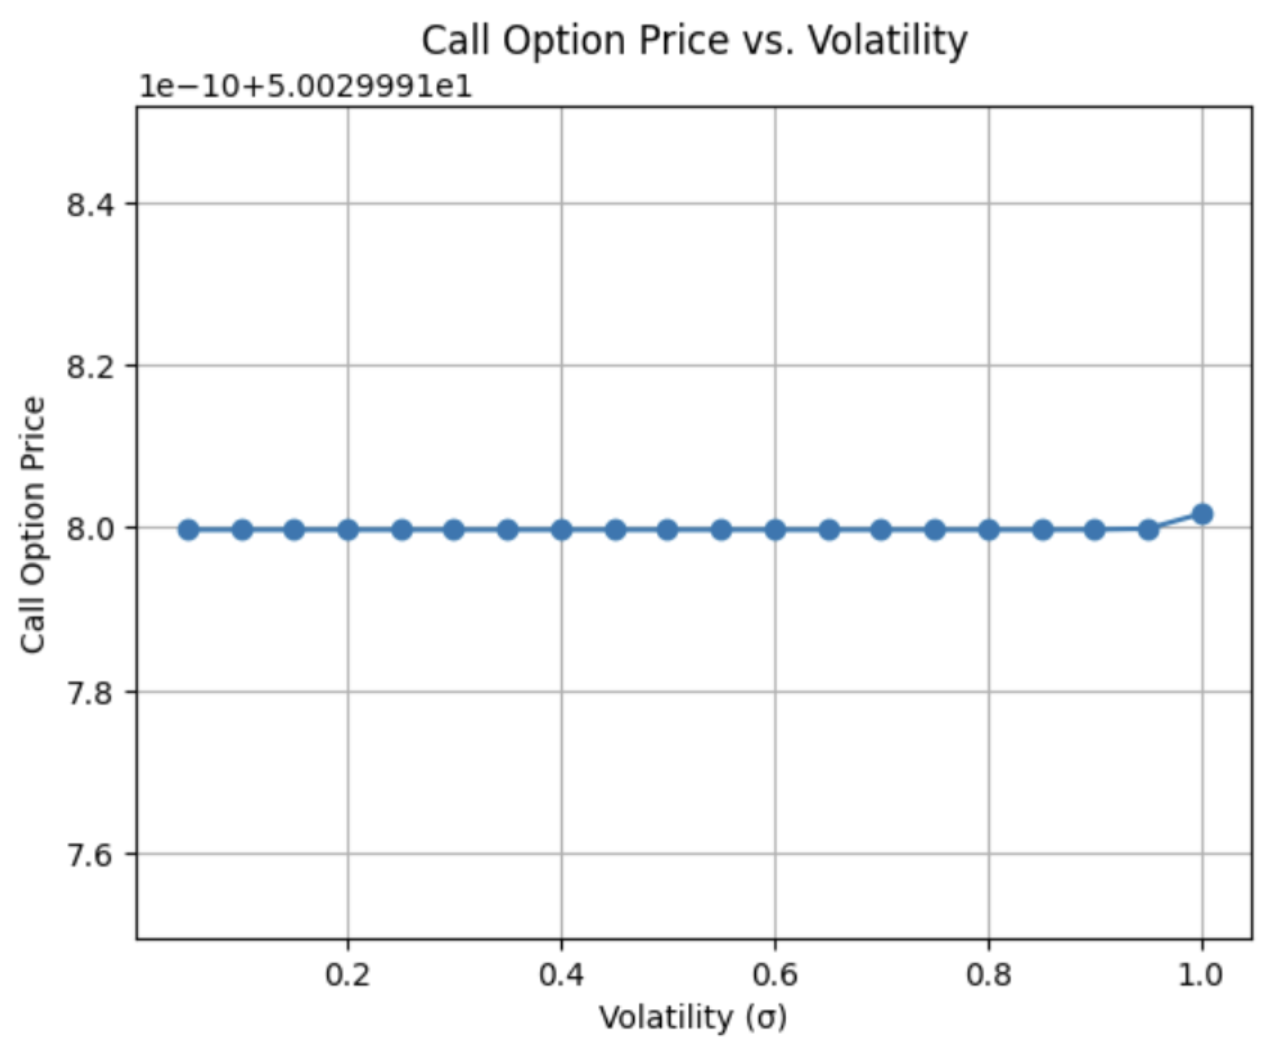
\includegraphics[width=\textwidth]{Screenshot 2024-06-06 at 9.27.11 PM.png}
    \caption{Call Option Price vs. Volatility}
\end{figure}


(b) Interpret the results.

\vspace{\baselineskip}


As volatility increases from .005 to 1 we do not see much change in the call 

option price.

\vspace{\baselineskip}

(c) Calculate the option price for \( \sigma = 5 \).

\vspace{\baselineskip}

Using the Google Colab code we see a signifcant increase in the call option 

price with c = \$64.00670002074642.

\end{document}